\documentclass[1p]{elsarticle_modified}
%\bibliographystyle{elsarticle-num}

%\usepackage[colorlinks]{hyperref}
%\usepackage{abbrmath_seonhwa} %\Abb, \Ascr, \Acal ,\Abf, \Afrak
\usepackage{amsfonts}
\usepackage{amssymb}
\usepackage{amsmath}
\usepackage{amsthm}
\usepackage{scalefnt}
\usepackage{amsbsy}
\usepackage{kotex}
\usepackage{caption}
\usepackage{subfig}
\usepackage{color}
\usepackage{graphicx}
\usepackage{xcolor} %% white, black, red, green, blue, cyan, magenta, yellow
\usepackage{float}
\usepackage{setspace}
\usepackage{hyperref}

\usepackage{tikz}
\usetikzlibrary{arrows}

\usepackage{multirow}
\usepackage{array} % fixed length table
\usepackage{hhline}

%%%%%%%%%%%%%%%%%%%%%
\makeatletter
\renewcommand*\env@matrix[1][\arraystretch]{%
	\edef\arraystretch{#1}%
	\hskip -\arraycolsep
	\let\@ifnextchar\new@ifnextchar
	\array{*\c@MaxMatrixCols c}}
\makeatother %https://tex.stackexchange.com/questions/14071/how-can-i-increase-the-line-spacing-in-a-matrix
%%%%%%%%%%%%%%%

\usepackage[normalem]{ulem}

\newcommand{\msout}[1]{\ifmmode\text{\sout{\ensuremath{#1}}}\else\sout{#1}\fi}
%SOURCE: \msout is \stkout macro in https://tex.stackexchange.com/questions/20609/strikeout-in-math-mode

\newcommand{\cancel}[1]{
	\ifmmode
	{\color{red}\msout{#1}}
	\else
	{\color{red}\sout{#1}}
	\fi
}

\newcommand{\add}[1]{
	{\color{blue}\uwave{#1}}
}

\newcommand{\replace}[2]{
	\ifmmode
	{\color{red}\msout{#1}}{\color{blue}\uwave{#2}}
	\else
	{\color{red}\sout{#1}}{\color{blue}\uwave{#2}}
	\fi
}

\newcommand{\Sol}{\mathcal{S}} %segment
\newcommand{\D}{D} %diagram
\newcommand{\A}{\mathcal{A}} %arc


%%%%%%%%%%%%%%%%%%%%%%%%%%%%%5 test

\def\sl{\operatorname{\textup{SL}}(2,\Cbb)}
\def\psl{\operatorname{\textup{PSL}}(2,\Cbb)}
\def\quan{\mkern 1mu \triangleright \mkern 1mu}

\theoremstyle{definition}
\newtheorem{thm}{Theorem}[section]
\newtheorem{prop}[thm]{Proposition}
\newtheorem{lem}[thm]{Lemma}
\newtheorem{ques}[thm]{Question}
\newtheorem{cor}[thm]{Corollary}
\newtheorem{defn}[thm]{Definition}
\newtheorem{exam}[thm]{Example}
\newtheorem{rmk}[thm]{Remark}
\newtheorem{alg}[thm]{Algorithm}

\newcommand{\I}{\sqrt{-1}}
\begin{document}

%\begin{frontmatter}
%
%\title{Boundary parabolic representations of knots up to 8 crossings}
%
%%% Group authors per affiliation:
%\author{Yunhi Cho} 
%\address{Department of Mathematics, University of Seoul, Seoul, Korea}
%\ead{yhcho@uos.ac.kr}
%
%
%\author{Seonhwa Kim} %\fnref{s_kim}}
%\address{Center for Geometry and Physics, Institute for Basic Science, Pohang, 37673, Korea}
%\ead{ryeona17@ibs.re.kr}
%
%\author{Hyuk Kim}
%\address{Department of Mathematical Sciences, Seoul National University, Seoul 08826, Korea}
%\ead{hyukkim@snu.ac.kr}
%
%\author{Seokbeom Yoon}
%\address{Department of Mathematical Sciences, Seoul National University, Seoul, 08826,  Korea}
%\ead{sbyoon15@snu.ac.kr}
%
%\begin{abstract}
%We find all boundary parabolic representation of knots up to 8 crossings.
%
%\end{abstract}
%\begin{keyword}
%    \MSC[2010] 57M25 
%\end{keyword}
%
%\end{frontmatter}

%\linenumbers
%\tableofcontents
%
\newcommand\colored[1]{\textcolor{white}{\rule[-0.35ex]{0.8em}{1.4ex}}\kern-0.8em\color{red} #1}%
%\newcommand\colored[1]{\textcolor{white}{ #1}\kern-2.17ex	\textcolor{white}{ #1}\kern-1.81ex	\textcolor{white}{ #1}\kern-2.15ex\color{red}#1	}

{\Large $\underline{12a_{0687}~(K12a_{0687})}$}

\setlength{\tabcolsep}{10pt}
\renewcommand{\arraystretch}{1.6}
\vspace{1cm}\begin{tabular}{m{100pt}>{\centering\arraybackslash}m{274pt}}
\multirow{5}{120pt}{
	\centering
	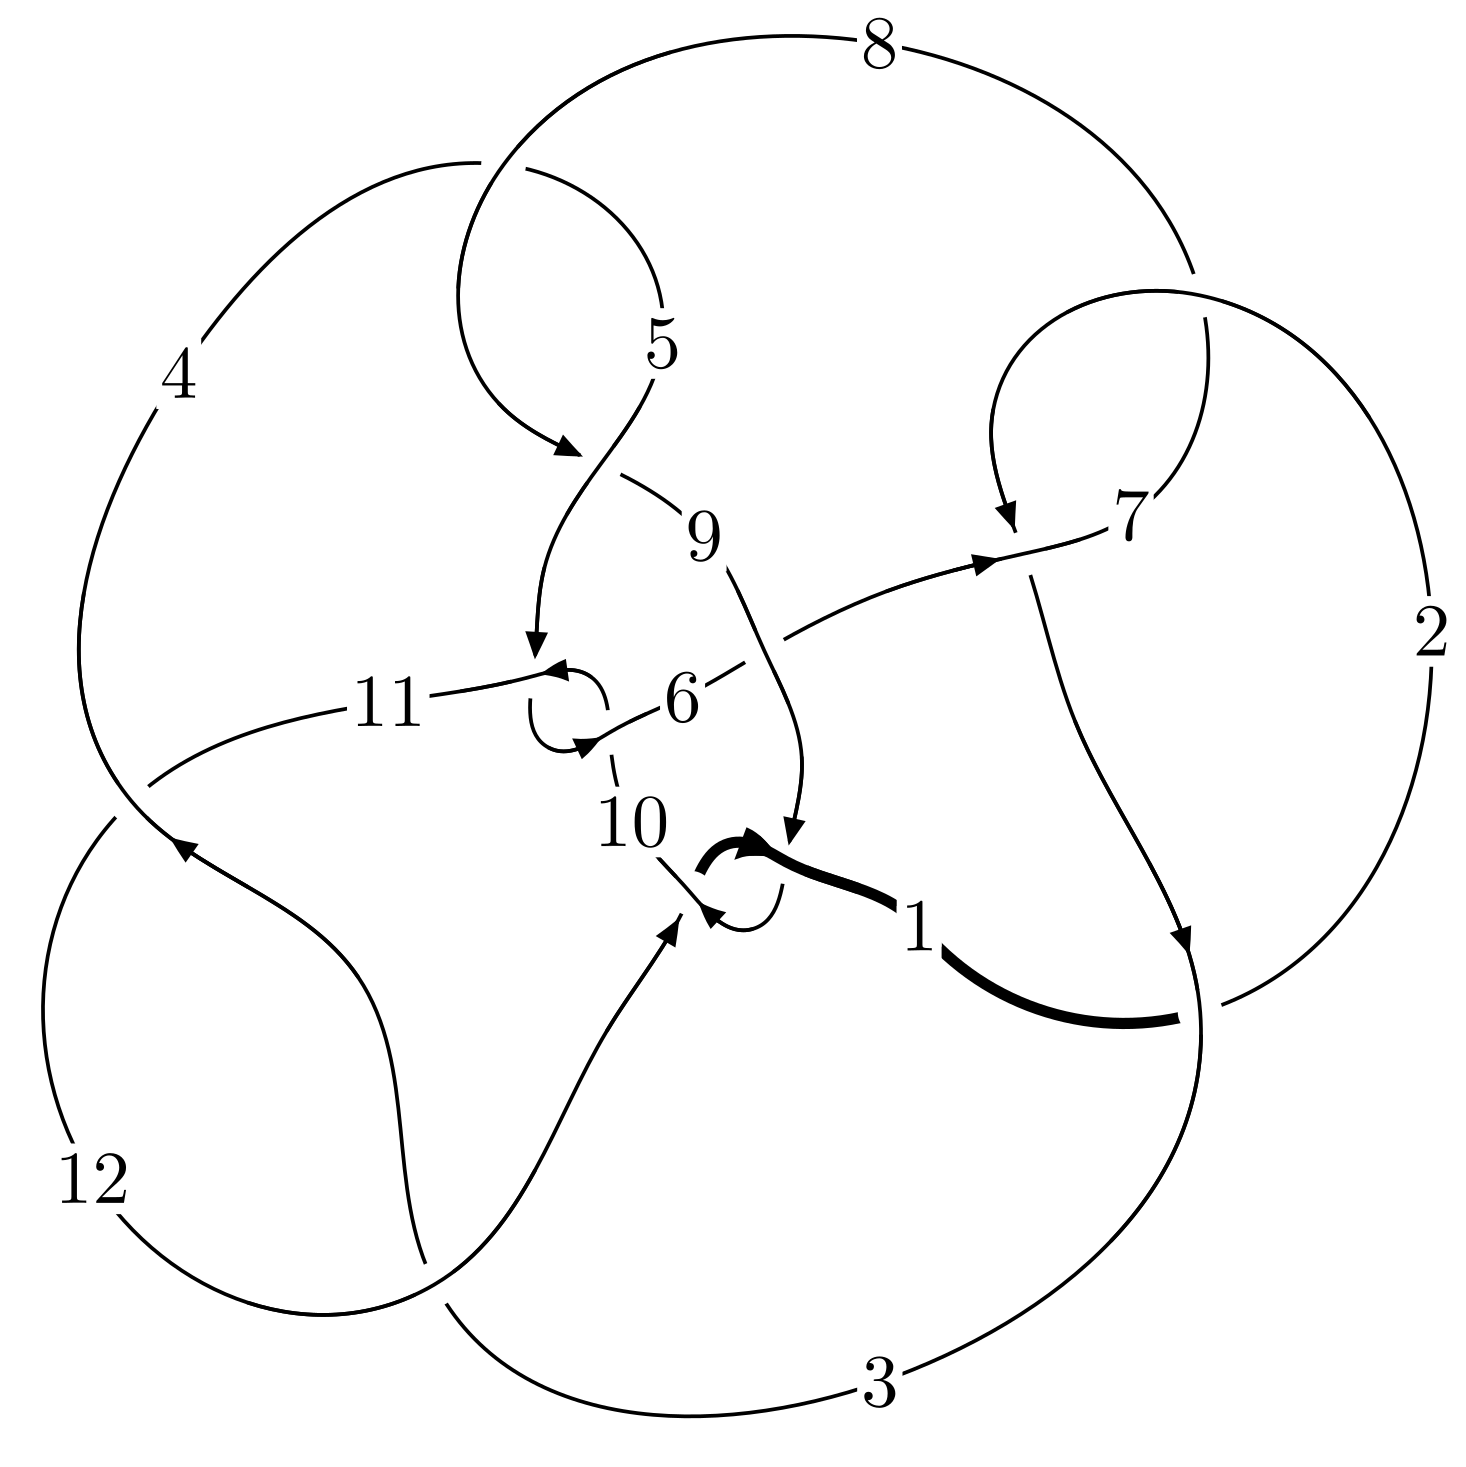
\includegraphics[width=112pt]{../../../GIT/diagram.site/Diagrams/png/1488_12a_0687.png}\\
\ \ \ A knot diagram\footnotemark}&
\allowdisplaybreaks
\textbf{Linearized knot diagam} \\
\cline{2-2}
 &
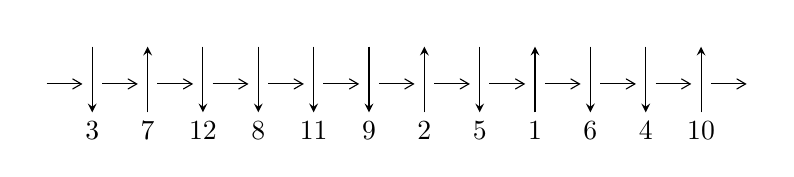
\begin{tikzpicture}[x=20pt, y=17pt]
	% nodes
	\node (C0) at (0, 0) {};
	\node (C1) at (1, 0) {};
	\node (C1U) at (1, +1) {};
	\node (C1D) at (1, -1) {3};

	\node (C2) at (2, 0) {};
	\node (C2U) at (2, +1) {};
	\node (C2D) at (2, -1) {7};

	\node (C3) at (3, 0) {};
	\node (C3U) at (3, +1) {};
	\node (C3D) at (3, -1) {12};

	\node (C4) at (4, 0) {};
	\node (C4U) at (4, +1) {};
	\node (C4D) at (4, -1) {8};

	\node (C5) at (5, 0) {};
	\node (C5U) at (5, +1) {};
	\node (C5D) at (5, -1) {11};

	\node (C6) at (6, 0) {};
	\node (C6U) at (6, +1) {};
	\node (C6D) at (6, -1) {9};

	\node (C7) at (7, 0) {};
	\node (C7U) at (7, +1) {};
	\node (C7D) at (7, -1) {2};

	\node (C8) at (8, 0) {};
	\node (C8U) at (8, +1) {};
	\node (C8D) at (8, -1) {5};

	\node (C9) at (9, 0) {};
	\node (C9U) at (9, +1) {};
	\node (C9D) at (9, -1) {1};

	\node (C10) at (10, 0) {};
	\node (C10U) at (10, +1) {};
	\node (C10D) at (10, -1) {6};

	\node (C11) at (11, 0) {};
	\node (C11U) at (11, +1) {};
	\node (C11D) at (11, -1) {4};

	\node (C12) at (12, 0) {};
	\node (C12U) at (12, +1) {};
	\node (C12D) at (12, -1) {10};
	\node (C13) at (13, 0) {};

	% arrows
	\draw[->,>={angle 60}]
	(C0) edge (C1) (C1) edge (C2) (C2) edge (C3) (C3) edge (C4) (C4) edge (C5) (C5) edge (C6) (C6) edge (C7) (C7) edge (C8) (C8) edge (C9) (C9) edge (C10) (C10) edge (C11) (C11) edge (C12) (C12) edge (C13) ;	\draw[->,>=stealth]
	(C1U) edge (C1D) (C2D) edge (C2U) (C3U) edge (C3D) (C4U) edge (C4D) (C5U) edge (C5D) (C6U) edge (C6D) (C7D) edge (C7U) (C8U) edge (C8D) (C9D) edge (C9U) (C10U) edge (C10D) (C11U) edge (C11D) (C12D) edge (C12U) ;
	\end{tikzpicture} \\
\hhline{~~} \\& 
\textbf{Solving Sequence} \\ \cline{2-2} 
 &
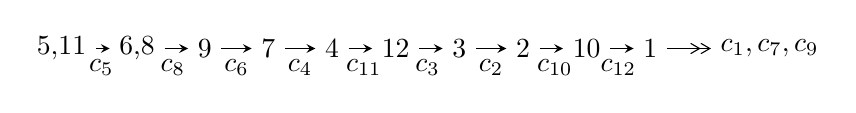
\begin{tikzpicture}[x=23pt, y=7pt]
	% node
	\node (A0) at (-1/8, 0) {5,11};
	\node (A1) at (17/16, 0) {6,8};
	\node (A2) at (17/8, 0) {9};
	\node (A3) at (25/8, 0) {7};
	\node (A4) at (33/8, 0) {4};
	\node (A5) at (41/8, 0) {12};
	\node (A6) at (49/8, 0) {3};
	\node (A7) at (57/8, 0) {2};
	\node (A8) at (65/8, 0) {10};
	\node (A9) at (73/8, 0) {1};
	\node (C1) at (1/2, -1) {$c_{5}$};
	\node (C2) at (13/8, -1) {$c_{8}$};
	\node (C3) at (21/8, -1) {$c_{6}$};
	\node (C4) at (29/8, -1) {$c_{4}$};
	\node (C5) at (37/8, -1) {$c_{11}$};
	\node (C6) at (45/8, -1) {$c_{3}$};
	\node (C7) at (53/8, -1) {$c_{2}$};
	\node (C8) at (61/8, -1) {$c_{10}$};
	\node (C9) at (69/8, -1) {$c_{12}$};
	\node (A10) at (11, 0) {$c_{1},c_{7},c_{9}$};

	% edge
	\draw[->,>=stealth]	
	(A0) edge (A1) (A1) edge (A2) (A2) edge (A3) (A3) edge (A4) (A4) edge (A5) (A5) edge (A6) (A6) edge (A7) (A7) edge (A8) (A8) edge (A9) ;
	\draw[->>,>={angle 60}]	
	(A9) edge (A10);
\end{tikzpicture} \\ 

\end{tabular} \\

\footnotetext{
The image of knot diagram is generated by the software ``\textbf{Draw programme}" developed by Andrew Bartholomew(\url{http://www.layer8.co.uk/maths/draw/index.htm\#Running-draw}), where we modified some parts for our purpose(\url{https://github.com/CATsTAILs/LinksPainter}).
}\phantom \\ \newline 
\centering \textbf{Ideals for irreducible components\footnotemark of $X_{\text{par}}$} 
 
\begin{align*}
I^u_{1}&=\langle 
-7.88489\times10^{881} u^{156}+5.04115\times10^{881} u^{155}+\cdots+1.36721\times10^{885} b+7.83741\times10^{885},\\
\phantom{I^u_{1}}&\phantom{= \langle  }1.51590\times10^{887} u^{156}+1.49559\times10^{887} u^{155}+\cdots+3.82955\times10^{888} a+1.83695\times10^{890},\\
\phantom{I^u_{1}}&\phantom{= \langle  }u^{157}+u^{156}+\cdots-13732 u+2801\rangle \\
I^u_{2}&=\langle 
6.98058\times10^{29} u^{45}+2.34056\times10^{31} u^{44}+\cdots+8.45573\times10^{29} b+5.19010\times10^{31},\\
\phantom{I^u_{2}}&\phantom{= \langle  }-1.05603\times10^{31} u^{45}+6.43040\times10^{31} u^{44}+\cdots+8.45573\times10^{29} a+1.26598\times10^{32},\\
\phantom{I^u_{2}}&\phantom{= \langle  }u^{46}+16 u^{44}+\cdots-2 u+1\rangle \\
\\
\end{align*}
\raggedright * 2 irreducible components of $\dim_{\mathbb{C}}=0$, with total 203 representations.\\
\footnotetext{All coefficients of polynomials are rational numbers. But the coefficients are sometimes approximated in decimal forms when there is not enough margin.}
\newpage
\renewcommand{\arraystretch}{1}
\centering \section*{I. $I^u_{1}= \langle -7.88\times10^{881} u^{156}+5.04\times10^{881} u^{155}+\cdots+1.37\times10^{885} b+7.84\times10^{885},\;1.52\times10^{887} u^{156}+1.50\times10^{887} u^{155}+\cdots+3.83\times10^{888} a+1.84\times10^{890},\;u^{157}+u^{156}+\cdots-13732 u+2801 \rangle$}
\flushleft \textbf{(i) Arc colorings}\\
\begin{tabular}{m{7pt} m{180pt} m{7pt} m{180pt} }
\flushright $a_{5}=$&$\begin{pmatrix}1\\0\end{pmatrix}$ \\
\flushright $a_{11}=$&$\begin{pmatrix}0\\u\end{pmatrix}$ \\
\flushright $a_{6}=$&$\begin{pmatrix}1\\u^2\end{pmatrix}$ \\
\flushright $a_{8}=$&$\begin{pmatrix}-0.0395843 u^{156}-0.0390538 u^{155}+\cdots+6.00367 u-47.9679\\0.000576714 u^{156}-0.000368718 u^{155}+\cdots+16.8195 u-5.73242\end{pmatrix}$ \\
\flushright $a_{9}=$&$\begin{pmatrix}-0.0401610 u^{156}-0.0386851 u^{155}+\cdots-10.8158 u-42.2355\\0.000576714 u^{156}-0.000368718 u^{155}+\cdots+16.8195 u-5.73242\end{pmatrix}$ \\
\flushright $a_{7}=$&$\begin{pmatrix}0.0292302 u^{156}+0.0194863 u^{155}+\cdots+288.828 u-15.3680\\-0.00382346 u^{156}+0.0105651 u^{155}+\cdots-249.524 u+42.7915\end{pmatrix}$ \\
\flushright $a_{4}=$&$\begin{pmatrix}-0.00864217 u^{156}-0.0147723 u^{155}+\cdots+8.42837 u-22.7494\\0.0132793 u^{156}-0.0288943 u^{155}+\cdots+805.874 u-143.749\end{pmatrix}$ \\
\flushright $a_{12}=$&$\begin{pmatrix}-0.0126184 u^{156}+0.0133006 u^{155}+\cdots-460.460 u+95.0835\\-0.0388728 u^{156}-0.0404769 u^{155}+\cdots+87.6322 u-45.1102\end{pmatrix}$ \\
\flushright $a_{3}=$&$\begin{pmatrix}0.0360791 u^{156}+0.0376727 u^{155}+\cdots+34.8247 u+5.35530\\0.0150618 u^{156}+0.00404137 u^{155}+\cdots+265.235 u-37.9961\end{pmatrix}$ \\
\flushright $a_{2}=$&$\begin{pmatrix}0.0142652 u^{156}-0.00878578 u^{155}+\cdots+398.926 u-78.0566\\-0.0136596 u^{156}-0.0457142 u^{155}+\cdots+646.176 u-134.161\end{pmatrix}$ \\
\flushright $a_{10}=$&$\begin{pmatrix}u\\u^3+u\end{pmatrix}$ \\
\flushright $a_{1}=$&$\begin{pmatrix}0.0143267 u^{156}+0.0367680 u^{155}+\cdots-444.852 u+111.218\\-0.0316780 u^{156}-0.0280375 u^{155}+\cdots-19.9885 u-19.2345\end{pmatrix}$\\&\end{tabular}
\flushleft \textbf{(ii) Obstruction class $= -1$}\\~\\
\flushleft \textbf{(iii) Cusp Shapes $= 0.0904845 u^{156}+0.0524635 u^{155}+\cdots+426.624 u-32.7175$}\\~\\
\newpage\renewcommand{\arraystretch}{1}
\flushleft \textbf{(iv) u-Polynomials at the component}\newline \\
\begin{tabular}{m{50pt}|m{274pt}}
Crossings & \hspace{64pt}u-Polynomials at each crossing \\
\hline $$\begin{aligned}c_{1}\end{aligned}$$&$\begin{aligned}
&u^{157}+75 u^{156}+\cdots-314997534 u-13845841
\end{aligned}$\\
\hline $$\begin{aligned}c_{2},c_{7}\end{aligned}$$&$\begin{aligned}
&u^{157}+u^{156}+\cdots+6588 u+3721
\end{aligned}$\\
\hline $$\begin{aligned}c_{3},c_{11}\end{aligned}$$&$\begin{aligned}
&u^{157}-4 u^{156}+\cdots+14174519 u-1906367
\end{aligned}$\\
\hline $$\begin{aligned}c_{4},c_{8}\end{aligned}$$&$\begin{aligned}
&u^{157}+3 u^{156}+\cdots+8 u+1
\end{aligned}$\\
\hline $$\begin{aligned}c_{5},c_{10}\end{aligned}$$&$\begin{aligned}
&u^{157}+u^{156}+\cdots-13732 u+2801
\end{aligned}$\\
\hline $$\begin{aligned}c_{6}\end{aligned}$$&$\begin{aligned}
&u^{157}-3 u^{156}+\cdots-346340 u+292121
\end{aligned}$\\
\hline $$\begin{aligned}c_{9},c_{12}\end{aligned}$$&$\begin{aligned}
&u^{157}+4 u^{156}+\cdots+13669 u+2263
\end{aligned}$\\
\hline
\end{tabular}\\~\\
\newpage\renewcommand{\arraystretch}{1}
\flushleft \textbf{(v) Riley Polynomials at the component}\newline \\
\begin{tabular}{m{50pt}|m{274pt}}
Crossings & \hspace{64pt}Riley Polynomials at each crossing \\
\hline $$\begin{aligned}c_{1}\end{aligned}$$&$\begin{aligned}
&y^{157}+39 y^{156}+\cdots-7046372593682426 y-191707312997281
\end{aligned}$\\
\hline $$\begin{aligned}c_{2},c_{7}\end{aligned}$$&$\begin{aligned}
&y^{157}+75 y^{156}+\cdots-314997534 y-13845841
\end{aligned}$\\
\hline $$\begin{aligned}c_{3},c_{11}\end{aligned}$$&$\begin{aligned}
&y^{157}+114 y^{156}+\cdots-60423847276045 y-3634235138689
\end{aligned}$\\
\hline $$\begin{aligned}c_{4},c_{8}\end{aligned}$$&$\begin{aligned}
&y^{157}-75 y^{156}+\cdots+6 y-1
\end{aligned}$\\
\hline $$\begin{aligned}c_{5},c_{10}\end{aligned}$$&$\begin{aligned}
&y^{157}+99 y^{156}+\cdots-1215170132 y-7845601
\end{aligned}$\\
\hline $$\begin{aligned}c_{6}\end{aligned}$$&$\begin{aligned}
&y^{157}-3 y^{156}+\cdots-13877806866712 y-85334678641
\end{aligned}$\\
\hline $$\begin{aligned}c_{9},c_{12}\end{aligned}$$&$\begin{aligned}
&y^{157}+78 y^{156}+\cdots-296376829 y-5121169
\end{aligned}$\\
\hline
\end{tabular}\\~\\
\newpage\flushleft \textbf{(vi) Complex Volumes and Cusp Shapes}
$$\begin{array}{c|c|c}  
\text{Solutions to }I^u_{1}& \I (\text{vol} + \sqrt{-1}CS) & \text{Cusp shape}\\
 \hline 
\begin{aligned}
u &= -0.983424 + 0.118249 I \\
a &= -1.292700 - 0.555427 I \\
b &= -1.021630 - 0.532125 I\end{aligned}
 & \phantom{-}2.09693 - 1.77887 I & \phantom{-0.000000 } 0 \\ \hline\begin{aligned}
u &= -0.983424 - 0.118249 I \\
a &= -1.292700 + 0.555427 I \\
b &= -1.021630 + 0.532125 I\end{aligned}
 & \phantom{-}2.09693 + 1.77887 I & \phantom{-0.000000 } 0 \\ \hline\begin{aligned}
u &= -0.953573 + 0.264717 I \\
a &= -1.39252 - 0.44034 I \\
b &= -0.477503 - 0.472794 I\end{aligned}
 & \phantom{-}1.38071 + 2.57286 I & \phantom{-0.000000 } 0 \\ \hline\begin{aligned}
u &= -0.953573 - 0.264717 I \\
a &= -1.39252 + 0.44034 I \\
b &= -0.477503 + 0.472794 I\end{aligned}
 & \phantom{-}1.38071 - 2.57286 I & \phantom{-0.000000 } 0 \\ \hline\begin{aligned}
u &= \phantom{-}0.646783 + 0.777333 I \\
a &= -1.035230 + 0.533846 I \\
b &= -1.064440 + 0.310838 I\end{aligned}
 & -2.42988 + 0.41909 I & \phantom{-0.000000 } 0 \\ \hline\begin{aligned}
u &= \phantom{-}0.646783 - 0.777333 I \\
a &= -1.035230 - 0.533846 I \\
b &= -1.064440 - 0.310838 I\end{aligned}
 & -2.42988 - 0.41909 I & \phantom{-0.000000 } 0 \\ \hline\begin{aligned}
u &= \phantom{-}0.962659 + 0.205398 I \\
a &= \phantom{-}1.209760 - 0.643836 I \\
b &= \phantom{-}1.146630 - 0.543092 I\end{aligned}
 & \phantom{-}0.74143 + 7.22667 I & \phantom{-0.000000 } 0 \\ \hline\begin{aligned}
u &= \phantom{-}0.962659 - 0.205398 I \\
a &= \phantom{-}1.209760 + 0.643836 I \\
b &= \phantom{-}1.146630 + 0.543092 I\end{aligned}
 & \phantom{-}0.74143 - 7.22667 I & \phantom{-0.000000 } 0 \\ \hline\begin{aligned}
u &= -0.320494 + 0.969075 I \\
a &= \phantom{-}0.051229 - 0.785137 I \\
b &= -1.034320 + 0.663947 I\end{aligned}
 & -4.31173 + 3.30916 I & \phantom{-0.000000 } 0 \\ \hline\begin{aligned}
u &= -0.320494 - 0.969075 I \\
a &= \phantom{-}0.051229 + 0.785137 I \\
b &= -1.034320 - 0.663947 I\end{aligned}
 & -4.31173 - 3.30916 I & \phantom{-0.000000 } 0\\
 \hline 
 \end{array}$$\newpage$$\begin{array}{c|c|c}  
\text{Solutions to }I^u_{1}& \I (\text{vol} + \sqrt{-1}CS) & \text{Cusp shape}\\
 \hline 
\begin{aligned}
u &= \phantom{-}0.517962 + 0.905954 I \\
a &= \phantom{-}1.07818 - 0.94510 I \\
b &= \phantom{-}0.076738 + 0.558359 I\end{aligned}
 & -0.18244 - 7.76232 I & \phantom{-0.000000 } 0 \\ \hline\begin{aligned}
u &= \phantom{-}0.517962 - 0.905954 I \\
a &= \phantom{-}1.07818 + 0.94510 I \\
b &= \phantom{-}0.076738 - 0.558359 I\end{aligned}
 & -0.18244 + 7.76232 I & \phantom{-0.000000 } 0 \\ \hline\begin{aligned}
u &= -0.125294 + 1.040410 I \\
a &= \phantom{-}0.0169154 + 0.0736309 I \\
b &= -0.28755 - 1.51200 I\end{aligned}
 & \phantom{-}3.81414 - 0.90830 I & \phantom{-0.000000 } 0 \\ \hline\begin{aligned}
u &= -0.125294 - 1.040410 I \\
a &= \phantom{-}0.0169154 - 0.0736309 I \\
b &= -0.28755 + 1.51200 I\end{aligned}
 & \phantom{-}3.81414 + 0.90830 I & \phantom{-0.000000 } 0 \\ \hline\begin{aligned}
u &= -0.050925 + 1.048040 I \\
a &= \phantom{-}0.142537 + 0.947115 I \\
b &= \phantom{-}0.355411 - 0.817437 I\end{aligned}
 & \phantom{-}3.47290 + 2.16111 I & \phantom{-0.000000 } 0 \\ \hline\begin{aligned}
u &= -0.050925 - 1.048040 I \\
a &= \phantom{-}0.142537 - 0.947115 I \\
b &= \phantom{-}0.355411 + 0.817437 I\end{aligned}
 & \phantom{-}3.47290 - 2.16111 I & \phantom{-0.000000 } 0 \\ \hline\begin{aligned}
u &= \phantom{-}0.506761 + 0.923868 I \\
a &= \phantom{-}1.24946 - 1.18931 I \\
b &= \phantom{-}1.005110 + 0.582922 I\end{aligned}
 & -1.95131 - 4.96181 I & \phantom{-0.000000 } 0 \\ \hline\begin{aligned}
u &= \phantom{-}0.506761 - 0.923868 I \\
a &= \phantom{-}1.24946 + 1.18931 I \\
b &= \phantom{-}1.005110 - 0.582922 I\end{aligned}
 & -1.95131 + 4.96181 I & \phantom{-0.000000 } 0 \\ \hline\begin{aligned}
u &= \phantom{-}0.816371 + 0.666474 I \\
a &= -0.549641 + 0.190487 I \\
b &= -0.877011 + 0.666561 I\end{aligned}
 & -3.67100 - 1.69687 I & \phantom{-0.000000 } 0 \\ \hline\begin{aligned}
u &= \phantom{-}0.816371 - 0.666474 I \\
a &= -0.549641 - 0.190487 I \\
b &= -0.877011 - 0.666561 I\end{aligned}
 & -3.67100 + 1.69687 I & \phantom{-0.000000 } 0\\
 \hline 
 \end{array}$$\newpage$$\begin{array}{c|c|c}  
\text{Solutions to }I^u_{1}& \I (\text{vol} + \sqrt{-1}CS) & \text{Cusp shape}\\
 \hline 
\begin{aligned}
u &= -0.484533 + 0.779590 I \\
a &= -0.354392 - 1.105070 I \\
b &= -1.237300 + 0.270956 I\end{aligned}
 & -4.40866 - 4.50850 I & \phantom{-0.000000 } 0 \\ \hline\begin{aligned}
u &= -0.484533 - 0.779590 I \\
a &= -0.354392 + 1.105070 I \\
b &= -1.237300 - 0.270956 I\end{aligned}
 & -4.40866 + 4.50850 I & \phantom{-0.000000 } 0 \\ \hline\begin{aligned}
u &= \phantom{-}0.134797 + 0.907142 I \\
a &= \phantom{-}2.13452 - 1.41578 I \\
b &= \phantom{-}1.053360 + 0.458463 I\end{aligned}
 & \phantom{-}3.79683 - 5.21301 I & \phantom{-0.000000 } 0 \\ \hline\begin{aligned}
u &= \phantom{-}0.134797 - 0.907142 I \\
a &= \phantom{-}2.13452 + 1.41578 I \\
b &= \phantom{-}1.053360 - 0.458463 I\end{aligned}
 & \phantom{-}3.79683 + 5.21301 I & \phantom{-0.000000 } 0 \\ \hline\begin{aligned}
u &= \phantom{-}0.151343 + 0.903789 I \\
a &= -1.41628 - 0.05456 I \\
b &= -1.49638 + 0.09674 I\end{aligned}
 & -1.23675 - 2.85908 I & \phantom{-0.000000 } 0 \\ \hline\begin{aligned}
u &= \phantom{-}0.151343 - 0.903789 I \\
a &= -1.41628 + 0.05456 I \\
b &= -1.49638 - 0.09674 I\end{aligned}
 & -1.23675 + 2.85908 I & \phantom{-0.000000 } 0 \\ \hline\begin{aligned}
u &= -0.088980 + 0.911104 I \\
a &= -2.22518 - 1.10650 I \\
b &= -1.073320 + 0.405134 I\end{aligned}
 & \phantom{-}3.90559 - 0.80435 I & \phantom{-0.000000 } 0 \\ \hline\begin{aligned}
u &= -0.088980 - 0.911104 I \\
a &= -2.22518 + 1.10650 I \\
b &= -1.073320 - 0.405134 I\end{aligned}
 & \phantom{-}3.90559 + 0.80435 I & \phantom{-0.000000 } 0 \\ \hline\begin{aligned}
u &= -0.129431 + 0.895829 I \\
a &= \phantom{-}0.248150 + 1.140630 I \\
b &= -0.049560 - 1.201590 I\end{aligned}
 & \phantom{-}3.28928 + 1.91897 I & \phantom{-0.000000 } 0 \\ \hline\begin{aligned}
u &= -0.129431 - 0.895829 I \\
a &= \phantom{-}0.248150 - 1.140630 I \\
b &= -0.049560 + 1.201590 I\end{aligned}
 & \phantom{-}3.28928 - 1.91897 I & \phantom{-0.000000 } 0\\
 \hline 
 \end{array}$$\newpage$$\begin{array}{c|c|c}  
\text{Solutions to }I^u_{1}& \I (\text{vol} + \sqrt{-1}CS) & \text{Cusp shape}\\
 \hline 
\begin{aligned}
u &= -0.612763 + 0.660646 I \\
a &= -1.56504 - 0.86691 I \\
b &= -1.138800 + 0.640935 I\end{aligned}
 & -4.18401 + 1.65000 I & \phantom{-0.000000 } 0 \\ \hline\begin{aligned}
u &= -0.612763 - 0.660646 I \\
a &= -1.56504 + 0.86691 I \\
b &= -1.138800 - 0.640935 I\end{aligned}
 & -4.18401 - 1.65000 I & \phantom{-0.000000 } 0 \\ \hline\begin{aligned}
u &= -0.219192 + 0.873736 I \\
a &= \phantom{-}1.133280 + 0.104372 I \\
b &= \phantom{-}1.72318 - 0.04282 I\end{aligned}
 & -4.54438 + 7.47305 I & \phantom{-0.000000 } 0 \\ \hline\begin{aligned}
u &= -0.219192 - 0.873736 I \\
a &= \phantom{-}1.133280 - 0.104372 I \\
b &= \phantom{-}1.72318 + 0.04282 I\end{aligned}
 & -4.54438 - 7.47305 I & \phantom{-0.000000 } 0 \\ \hline\begin{aligned}
u &= -0.382410 + 0.797108 I \\
a &= -1.09618 - 0.93984 I \\
b &= \phantom{-}0.154925 + 0.411991 I\end{aligned}
 & \phantom{-}0.87708 + 2.51431 I & \phantom{-0.000000 } 0 \\ \hline\begin{aligned}
u &= -0.382410 - 0.797108 I \\
a &= -1.09618 + 0.93984 I \\
b &= \phantom{-}0.154925 - 0.411991 I\end{aligned}
 & \phantom{-}0.87708 - 2.51431 I & \phantom{-0.000000 } 0 \\ \hline\begin{aligned}
u &= \phantom{-}0.526170 + 0.706597 I \\
a &= -0.186604 - 0.941652 I \\
b &= -0.386499 + 0.260859 I\end{aligned}
 & -4.41300 - 2.16123 I & \phantom{-0.000000 } 0 \\ \hline\begin{aligned}
u &= \phantom{-}0.526170 - 0.706597 I \\
a &= -0.186604 + 0.941652 I \\
b &= -0.386499 - 0.260859 I\end{aligned}
 & -4.41300 + 2.16123 I & \phantom{-0.000000 } 0 \\ \hline\begin{aligned}
u &= \phantom{-}0.236131 + 0.830375 I \\
a &= -0.214590 - 1.160790 I \\
b &= \phantom{-}0.898111 + 0.411853 I\end{aligned}
 & -1.20612 + 0.95128 I & \phantom{-0.000000 } 0 \\ \hline\begin{aligned}
u &= \phantom{-}0.236131 - 0.830375 I \\
a &= -0.214590 + 1.160790 I \\
b &= \phantom{-}0.898111 - 0.411853 I\end{aligned}
 & -1.20612 - 0.95128 I & \phantom{-0.000000 } 0\\
 \hline 
 \end{array}$$\newpage$$\begin{array}{c|c|c}  
\text{Solutions to }I^u_{1}& \I (\text{vol} + \sqrt{-1}CS) & \text{Cusp shape}\\
 \hline 
\begin{aligned}
u &= -1.056910 + 0.426045 I \\
a &= \phantom{-}1.378430 - 0.183130 I \\
b &= \phantom{-}1.176020 + 0.065926 I\end{aligned}
 & -8.95915 + 1.30472 I & \phantom{-0.000000 } 0 \\ \hline\begin{aligned}
u &= -1.056910 - 0.426045 I \\
a &= \phantom{-}1.378430 + 0.183130 I \\
b &= \phantom{-}1.176020 - 0.065926 I\end{aligned}
 & -8.95915 - 1.30472 I & \phantom{-0.000000 } 0 \\ \hline\begin{aligned}
u &= -0.854770 + 0.762921 I \\
a &= \phantom{-}0.606990 + 0.356542 I \\
b &= \phantom{-}1.107180 + 0.636268 I\end{aligned}
 & -4.12077 - 1.72135 I & \phantom{-0.000000 } 0 \\ \hline\begin{aligned}
u &= -0.854770 - 0.762921 I \\
a &= \phantom{-}0.606990 - 0.356542 I \\
b &= \phantom{-}1.107180 - 0.636268 I\end{aligned}
 & -4.12077 + 1.72135 I & \phantom{-0.000000 } 0 \\ \hline\begin{aligned}
u &= \phantom{-}0.407873 + 1.071970 I \\
a &= -0.636057 + 0.959108 I \\
b &= -1.037400 - 0.218361 I\end{aligned}
 & -1.73344 - 0.63595 I & \phantom{-0.000000 } 0 \\ \hline\begin{aligned}
u &= \phantom{-}0.407873 - 1.071970 I \\
a &= -0.636057 - 0.959108 I \\
b &= -1.037400 + 0.218361 I\end{aligned}
 & -1.73344 + 0.63595 I & \phantom{-0.000000 } 0 \\ \hline\begin{aligned}
u &= -0.745385 + 0.876961 I \\
a &= -1.23068 - 0.81672 I \\
b &= -0.981818 + 0.850390 I\end{aligned}
 & -3.74907 + 7.62415 I & \phantom{-0.000000 } 0 \\ \hline\begin{aligned}
u &= -0.745385 - 0.876961 I \\
a &= -1.23068 + 0.81672 I \\
b &= -0.981818 - 0.850390 I\end{aligned}
 & -3.74907 - 7.62415 I & \phantom{-0.000000 } 0 \\ \hline\begin{aligned}
u &= -0.746880 + 0.880965 I \\
a &= \phantom{-}0.742828 + 0.555113 I \\
b &= \phantom{-}1.218590 + 0.372567 I\end{aligned}
 & -3.66009 + 3.61781 I & \phantom{-0.000000 } 0 \\ \hline\begin{aligned}
u &= -0.746880 - 0.880965 I \\
a &= \phantom{-}0.742828 - 0.555113 I \\
b &= \phantom{-}1.218590 - 0.372567 I\end{aligned}
 & -3.66009 - 3.61781 I & \phantom{-0.000000 } 0\\
 \hline 
 \end{array}$$\newpage$$\begin{array}{c|c|c}  
\text{Solutions to }I^u_{1}& \I (\text{vol} + \sqrt{-1}CS) & \text{Cusp shape}\\
 \hline 
\begin{aligned}
u &= -0.131246 + 0.823567 I \\
a &= \phantom{-}1.194740 - 0.415293 I \\
b &= \phantom{-}1.57754 + 0.38551 I\end{aligned}
 & -5.20350 - 1.29361 I & \phantom{-0.000000 } 0 \\ \hline\begin{aligned}
u &= -0.131246 - 0.823567 I \\
a &= \phantom{-}1.194740 + 0.415293 I \\
b &= \phantom{-}1.57754 - 0.38551 I\end{aligned}
 & -5.20350 + 1.29361 I & \phantom{-0.000000 } 0 \\ \hline\begin{aligned}
u &= -0.376515 + 1.110300 I \\
a &= \phantom{-}0.0180237 - 0.0417333 I \\
b &= -0.66910 - 1.31854 I\end{aligned}
 & \phantom{-}6.11212 + 5.28335 I & \phantom{-0.000000 } 0 \\ \hline\begin{aligned}
u &= -0.376515 - 1.110300 I \\
a &= \phantom{-}0.0180237 + 0.0417333 I \\
b &= -0.66910 + 1.31854 I\end{aligned}
 & \phantom{-}6.11212 - 5.28335 I & \phantom{-0.000000 } 0 \\ \hline\begin{aligned}
u &= \phantom{-}0.708612 + 0.956040 I \\
a &= \phantom{-}1.13424 - 0.86547 I \\
b &= \phantom{-}0.780133 + 0.804599 I\end{aligned}
 & -2.84437 - 3.98936 I & \phantom{-0.000000 } 0 \\ \hline\begin{aligned}
u &= \phantom{-}0.708612 - 0.956040 I \\
a &= \phantom{-}1.13424 + 0.86547 I \\
b &= \phantom{-}0.780133 - 0.804599 I\end{aligned}
 & -2.84437 + 3.98936 I & \phantom{-0.000000 } 0 \\ \hline\begin{aligned}
u &= \phantom{-}0.130319 + 1.185510 I \\
a &= -1.67725 + 1.17605 I \\
b &= -1.033190 - 0.359624 I\end{aligned}
 & \phantom{-}3.25928 - 2.97909 I & \phantom{-0.000000 } 0 \\ \hline\begin{aligned}
u &= \phantom{-}0.130319 - 1.185510 I \\
a &= -1.67725 - 1.17605 I \\
b &= -1.033190 + 0.359624 I\end{aligned}
 & \phantom{-}3.25928 + 2.97909 I & \phantom{-0.000000 } 0 \\ \hline\begin{aligned}
u &= \phantom{-}0.727293 + 0.347210 I \\
a &= -1.64949 - 0.12002 I \\
b &= -1.185650 + 0.272617 I\end{aligned}
 & -4.01071 + 2.09725 I & \phantom{-0.000000 } 0 \\ \hline\begin{aligned}
u &= \phantom{-}0.727293 - 0.347210 I \\
a &= -1.64949 + 0.12002 I \\
b &= -1.185650 - 0.272617 I\end{aligned}
 & -4.01071 - 2.09725 I & \phantom{-0.000000 } 0\\
 \hline 
 \end{array}$$\newpage$$\begin{array}{c|c|c}  
\text{Solutions to }I^u_{1}& \I (\text{vol} + \sqrt{-1}CS) & \text{Cusp shape}\\
 \hline 
\begin{aligned}
u &= -0.252364 + 1.169570 I \\
a &= \phantom{-}0.543026 + 0.868177 I \\
b &= \phantom{-}0.993662 - 0.576624 I\end{aligned}
 & \phantom{-}1.88635 + 2.96312 I & \phantom{-0.000000 } 0 \\ \hline\begin{aligned}
u &= -0.252364 - 1.169570 I \\
a &= \phantom{-}0.543026 - 0.868177 I \\
b &= \phantom{-}0.993662 + 0.576624 I\end{aligned}
 & \phantom{-}1.88635 - 2.96312 I & \phantom{-0.000000 } 0 \\ \hline\begin{aligned}
u &= -0.777869 + 0.932844 I \\
a &= -1.73517 - 0.15009 I \\
b &= -1.011600 + 0.477461 I\end{aligned}
 & \phantom{-}4.02418 + 1.15616 I & \phantom{-0.000000 } 0 \\ \hline\begin{aligned}
u &= -0.777869 - 0.932844 I \\
a &= -1.73517 + 0.15009 I \\
b &= -1.011600 - 0.477461 I\end{aligned}
 & \phantom{-}4.02418 - 1.15616 I & \phantom{-0.000000 } 0 \\ \hline\begin{aligned}
u &= \phantom{-}0.770158 + 0.143087 I \\
a &= \phantom{-}1.61615 - 0.26926 I \\
b &= \phantom{-}0.182574 - 0.638116 I\end{aligned}
 & -0.29177 - 8.18913 I & \phantom{-0.000000 } 0 \\ \hline\begin{aligned}
u &= \phantom{-}0.770158 - 0.143087 I \\
a &= \phantom{-}1.61615 + 0.26926 I \\
b &= \phantom{-}0.182574 + 0.638116 I\end{aligned}
 & -0.29177 + 8.18913 I & \phantom{-0.000000 } 0 \\ \hline\begin{aligned}
u &= -0.745739 + 0.150142 I \\
a &= \phantom{-}1.64583 - 0.38540 I \\
b &= \phantom{-}1.310780 + 0.301679 I\end{aligned}
 & -6.51205 - 7.33858 I & \phantom{-0.000000 } 0 \\ \hline\begin{aligned}
u &= -0.745739 - 0.150142 I \\
a &= \phantom{-}1.64583 + 0.38540 I \\
b &= \phantom{-}1.310780 - 0.301679 I\end{aligned}
 & -6.51205 + 7.33858 I & \phantom{-0.000000 } 0 \\ \hline\begin{aligned}
u &= \phantom{-}0.325677 + 0.687118 I \\
a &= \phantom{-}1.50972 - 2.19629 I \\
b &= -0.238481 + 0.091283 I\end{aligned}
 & -0.19815 - 7.87590 I & \phantom{-0.000000 } 0 \\ \hline\begin{aligned}
u &= \phantom{-}0.325677 - 0.687118 I \\
a &= \phantom{-}1.50972 + 2.19629 I \\
b &= -0.238481 - 0.091283 I\end{aligned}
 & -0.19815 + 7.87590 I & \phantom{-0.000000 } 0\\
 \hline 
 \end{array}$$\newpage$$\begin{array}{c|c|c}  
\text{Solutions to }I^u_{1}& \I (\text{vol} + \sqrt{-1}CS) & \text{Cusp shape}\\
 \hline 
\begin{aligned}
u &= \phantom{-}0.626984 + 0.406452 I \\
a &= \phantom{-}1.08105 - 1.25584 I \\
b &= \phantom{-}1.183510 - 0.175680 I\end{aligned}
 & -2.66699 + 2.02776 I & \phantom{-0.000000 } 0 \\ \hline\begin{aligned}
u &= \phantom{-}0.626984 - 0.406452 I \\
a &= \phantom{-}1.08105 + 1.25584 I \\
b &= \phantom{-}1.183510 + 0.175680 I\end{aligned}
 & -2.66699 - 2.02776 I & \phantom{-0.000000 } 0 \\ \hline\begin{aligned}
u &= -0.133704 + 1.245720 I \\
a &= \phantom{-}1.42031 + 1.39062 I \\
b &= \phantom{-}0.999596 - 0.472247 I\end{aligned}
 & \phantom{-}2.80674 + 7.95594 I & \phantom{-0.000000 } 0 \\ \hline\begin{aligned}
u &= -0.133704 - 1.245720 I \\
a &= \phantom{-}1.42031 - 1.39062 I \\
b &= \phantom{-}0.999596 + 0.472247 I\end{aligned}
 & \phantom{-}2.80674 - 7.95594 I & \phantom{-0.000000 } 0 \\ \hline\begin{aligned}
u &= \phantom{-}0.339817 + 1.214920 I \\
a &= \phantom{-}0.0407385 - 0.0339113 I \\
b &= \phantom{-}0.617308 - 1.167720 I\end{aligned}
 & \phantom{-}7.66052 - 0.37824 I & \phantom{-0.000000 } 0 \\ \hline\begin{aligned}
u &= \phantom{-}0.339817 - 1.214920 I \\
a &= \phantom{-}0.0407385 + 0.0339113 I \\
b &= \phantom{-}0.617308 + 1.167720 I\end{aligned}
 & \phantom{-}7.66052 + 0.37824 I & \phantom{-0.000000 } 0 \\ \hline\begin{aligned}
u &= \phantom{-}0.640165 + 0.365956 I \\
a &= -0.054069 + 0.221356 I \\
b &= -0.213191 + 0.801677 I\end{aligned}
 & -1.75066 + 3.45252 I & \phantom{-0.000000 } 0 \\ \hline\begin{aligned}
u &= \phantom{-}0.640165 - 0.365956 I \\
a &= -0.054069 - 0.221356 I \\
b &= -0.213191 - 0.801677 I\end{aligned}
 & -1.75066 - 3.45252 I & \phantom{-0.000000 } 0 \\ \hline\begin{aligned}
u &= \phantom{-}0.426623 + 1.190150 I \\
a &= -1.151290 + 0.678879 I \\
b &= -1.32224 - 0.59496 I\end{aligned}
 & -0.15983 - 6.07472 I & \phantom{-0.000000 } 0 \\ \hline\begin{aligned}
u &= \phantom{-}0.426623 - 1.190150 I \\
a &= -1.151290 - 0.678879 I \\
b &= -1.32224 + 0.59496 I\end{aligned}
 & -0.15983 + 6.07472 I & \phantom{-0.000000 } 0\\
 \hline 
 \end{array}$$\newpage$$\begin{array}{c|c|c}  
\text{Solutions to }I^u_{1}& \I (\text{vol} + \sqrt{-1}CS) & \text{Cusp shape}\\
 \hline 
\begin{aligned}
u &= \phantom{-}0.021040 + 1.272170 I \\
a &= -0.693871 + 0.166719 I \\
b &= \phantom{-}0.536816 + 0.380747 I\end{aligned}
 & \phantom{-}5.49007 + 1.49266 I & \phantom{-0.000000 } 0 \\ \hline\begin{aligned}
u &= \phantom{-}0.021040 - 1.272170 I \\
a &= -0.693871 - 0.166719 I \\
b &= \phantom{-}0.536816 - 0.380747 I\end{aligned}
 & \phantom{-}5.49007 - 1.49266 I & \phantom{-0.000000 } 0 \\ \hline\begin{aligned}
u &= \phantom{-}0.452878 + 1.191700 I \\
a &= \phantom{-}0.70334 - 1.32291 I \\
b &= \phantom{-}1.073640 + 0.500654 I\end{aligned}
 & -1.30030 - 6.59027 I & \phantom{-0.000000 } 0 \\ \hline\begin{aligned}
u &= \phantom{-}0.452878 - 1.191700 I \\
a &= \phantom{-}0.70334 + 1.32291 I \\
b &= \phantom{-}1.073640 - 0.500654 I\end{aligned}
 & -1.30030 + 6.59027 I & \phantom{-0.000000 } 0 \\ \hline\begin{aligned}
u &= \phantom{-}0.712829 + 0.112855 I \\
a &= \phantom{-}1.76416 - 0.04418 I \\
b &= \phantom{-}1.233130 + 0.188271 I\end{aligned}
 & -4.45501 - 3.38045 I & \phantom{-0.000000 } 0 \\ \hline\begin{aligned}
u &= \phantom{-}0.712829 - 0.112855 I \\
a &= \phantom{-}1.76416 + 0.04418 I \\
b &= \phantom{-}1.233130 - 0.188271 I\end{aligned}
 & -4.45501 + 3.38045 I & \phantom{-0.000000 } 0 \\ \hline\begin{aligned}
u &= \phantom{-}0.330624 + 1.262430 I \\
a &= -0.653500 + 0.923207 I \\
b &= -1.196400 - 0.536399 I\end{aligned}
 & -0.24784 - 7.12635 I & \phantom{-0.000000 } 0 \\ \hline\begin{aligned}
u &= \phantom{-}0.330624 - 1.262430 I \\
a &= -0.653500 - 0.923207 I \\
b &= -1.196400 + 0.536399 I\end{aligned}
 & -0.24784 + 7.12635 I & \phantom{-0.000000 } 0 \\ \hline\begin{aligned}
u &= \phantom{-}0.367802 + 1.252950 I \\
a &= -0.0958780 - 0.0426635 I \\
b &= -0.094302 + 1.077110 I\end{aligned}
 & \phantom{-}0.22235 - 4.50979 I & \phantom{-0.000000 } 0 \\ \hline\begin{aligned}
u &= \phantom{-}0.367802 - 1.252950 I \\
a &= -0.0958780 + 0.0426635 I \\
b &= -0.094302 - 1.077110 I\end{aligned}
 & \phantom{-}0.22235 + 4.50979 I & \phantom{-0.000000 } 0\\
 \hline 
 \end{array}$$\newpage$$\begin{array}{c|c|c}  
\text{Solutions to }I^u_{1}& \I (\text{vol} + \sqrt{-1}CS) & \text{Cusp shape}\\
 \hline 
\begin{aligned}
u &= -0.237519 + 0.641854 I \\
a &= -1.73385 - 1.69987 I \\
b &= \phantom{-}0.310537 + 0.119313 I\end{aligned}
 & \phantom{-}0.89751 + 2.53711 I & \phantom{-0.000000 } 0 \\ \hline\begin{aligned}
u &= -0.237519 - 0.641854 I \\
a &= -1.73385 + 1.69987 I \\
b &= \phantom{-}0.310537 - 0.119313 I\end{aligned}
 & \phantom{-}0.89751 - 2.53711 I & \phantom{-0.000000 } 0 \\ \hline\begin{aligned}
u &= \phantom{-}1.295290 + 0.267673 I \\
a &= -1.276210 + 0.365122 I \\
b &= -1.032390 + 0.509616 I\end{aligned}
 & -0.24810 + 6.75844 I & \phantom{-0.000000 } 0 \\ \hline\begin{aligned}
u &= \phantom{-}1.295290 - 0.267673 I \\
a &= -1.276210 - 0.365122 I \\
b &= -1.032390 - 0.509616 I\end{aligned}
 & -0.24810 - 6.75844 I & \phantom{-0.000000 } 0 \\ \hline\begin{aligned}
u &= -0.245529 + 1.303530 I \\
a &= \phantom{-}0.95196 + 1.09592 I \\
b &= \phantom{-}1.157910 - 0.593512 I\end{aligned}
 & \phantom{-}0.96053 + 3.93024 I & \phantom{-0.000000 } 0 \\ \hline\begin{aligned}
u &= -0.245529 - 1.303530 I \\
a &= \phantom{-}0.95196 - 1.09592 I \\
b &= \phantom{-}1.157910 + 0.593512 I\end{aligned}
 & \phantom{-}0.96053 - 3.93024 I & \phantom{-0.000000 } 0 \\ \hline\begin{aligned}
u &= -1.321120 + 0.163287 I \\
a &= \phantom{-}1.275800 + 0.314006 I \\
b &= \phantom{-}1.130950 + 0.531846 I\end{aligned}
 & -2.85813 - 12.78990 I & \phantom{-0.000000 } 0 \\ \hline\begin{aligned}
u &= -1.321120 - 0.163287 I \\
a &= \phantom{-}1.275800 - 0.314006 I \\
b &= \phantom{-}1.130950 - 0.531846 I\end{aligned}
 & -2.85813 + 12.78990 I & \phantom{-0.000000 } 0 \\ \hline\begin{aligned}
u &= -0.449007 + 1.272460 I \\
a &= -0.540863 - 1.263800 I \\
b &= -1.130470 + 0.491770 I\end{aligned}
 & -2.97284 + 11.87020 I & \phantom{-0.000000 } 0 \\ \hline\begin{aligned}
u &= -0.449007 - 1.272460 I \\
a &= -0.540863 + 1.263800 I \\
b &= -1.130470 - 0.491770 I\end{aligned}
 & -2.97284 - 11.87020 I & \phantom{-0.000000 } 0\\
 \hline 
 \end{array}$$\newpage$$\begin{array}{c|c|c}  
\text{Solutions to }I^u_{1}& \I (\text{vol} + \sqrt{-1}CS) & \text{Cusp shape}\\
 \hline 
\begin{aligned}
u &= \phantom{-}0.459011 + 1.277780 I \\
a &= \phantom{-}0.0366481 + 0.0116698 I \\
b &= -0.422203 + 1.233630 I\end{aligned}
 & \phantom{-}3.77311 - 12.74680 I & \phantom{-0.000000 } 0 \\ \hline\begin{aligned}
u &= \phantom{-}0.459011 - 1.277780 I \\
a &= \phantom{-}0.0366481 - 0.0116698 I \\
b &= -0.422203 - 1.233630 I\end{aligned}
 & \phantom{-}3.77311 + 12.74680 I & \phantom{-0.000000 } 0 \\ \hline\begin{aligned}
u &= \phantom{-}0.038501 + 1.364540 I \\
a &= -0.172701 + 0.331003 I \\
b &= \phantom{-}0.143783 - 0.895306 I\end{aligned}
 & \phantom{-}3.79424 + 1.41084 I & \phantom{-0.000000 } 0 \\ \hline\begin{aligned}
u &= \phantom{-}0.038501 - 1.364540 I \\
a &= -0.172701 - 0.331003 I \\
b &= \phantom{-}0.143783 + 0.895306 I\end{aligned}
 & \phantom{-}3.79424 - 1.41084 I & \phantom{-0.000000 } 0 \\ \hline\begin{aligned}
u &= \phantom{-}0.747351 + 1.143850 I \\
a &= \phantom{-}1.59189 - 0.40142 I \\
b &= \phantom{-}1.078190 + 0.539924 I\end{aligned}
 & \phantom{-}4.99973 - 7.83611 I & \phantom{-0.000000 } 0 \\ \hline\begin{aligned}
u &= \phantom{-}0.747351 - 1.143850 I \\
a &= \phantom{-}1.59189 + 0.40142 I \\
b &= \phantom{-}1.078190 - 0.539924 I\end{aligned}
 & \phantom{-}4.99973 + 7.83611 I & \phantom{-0.000000 } 0 \\ \hline\begin{aligned}
u &= \phantom{-}0.052669 + 1.366980 I \\
a &= \phantom{-}0.530681 + 0.354263 I \\
b &= -0.654916 + 0.209060 I\end{aligned}
 & \phantom{-}5.66080 + 3.73994 I & \phantom{-0.000000 } 0 \\ \hline\begin{aligned}
u &= \phantom{-}0.052669 - 1.366980 I \\
a &= \phantom{-}0.530681 - 0.354263 I \\
b &= -0.654916 - 0.209060 I\end{aligned}
 & \phantom{-}5.66080 - 3.73994 I & \phantom{-0.000000 } 0 \\ \hline\begin{aligned}
u &= -0.432461 + 1.298810 I \\
a &= \phantom{-}0.0011687 + 0.0425140 I \\
b &= \phantom{-}0.403576 + 1.111300 I\end{aligned}
 & \phantom{-}5.93690 + 7.16886 I & \phantom{-0.000000 } 0 \\ \hline\begin{aligned}
u &= -0.432461 - 1.298810 I \\
a &= \phantom{-}0.0011687 - 0.0425140 I \\
b &= \phantom{-}0.403576 - 1.111300 I\end{aligned}
 & \phantom{-}5.93690 - 7.16886 I & \phantom{-0.000000 } 0\\
 \hline 
 \end{array}$$\newpage$$\begin{array}{c|c|c}  
\text{Solutions to }I^u_{1}& \I (\text{vol} + \sqrt{-1}CS) & \text{Cusp shape}\\
 \hline 
\begin{aligned}
u &= \phantom{-}0.583237 + 1.254380 I \\
a &= -1.157820 + 0.720669 I \\
b &= -1.26101 - 0.81969 I\end{aligned}
 & \phantom{-}3.95794 - 12.84080 I & \phantom{-0.000000 } 0 \\ \hline\begin{aligned}
u &= \phantom{-}0.583237 - 1.254380 I \\
a &= -1.157820 - 0.720669 I \\
b &= -1.26101 + 0.81969 I\end{aligned}
 & \phantom{-}3.95794 + 12.84080 I & \phantom{-0.000000 } 0 \\ \hline\begin{aligned}
u &= -0.558556 + 1.279010 I \\
a &= \phantom{-}1.186450 + 0.705371 I \\
b &= \phantom{-}1.20369 - 0.77248 I\end{aligned}
 & \phantom{-}5.64130 + 7.32574 I & \phantom{-0.000000 } 0 \\ \hline\begin{aligned}
u &= -0.558556 - 1.279010 I \\
a &= \phantom{-}1.186450 - 0.705371 I \\
b &= \phantom{-}1.20369 + 0.77248 I\end{aligned}
 & \phantom{-}5.64130 - 7.32574 I & \phantom{-0.000000 } 0 \\ \hline\begin{aligned}
u &= -0.600972\phantom{ +0.000000I} \\
a &= -1.58786\phantom{ +0.000000I} \\
b &= -0.987414\phantom{ +0.000000I}\end{aligned}
 & -1.63262\phantom{ +0.000000I} & -5.64780\phantom{ +0.000000I} \\ \hline\begin{aligned}
u &= -0.650780 + 1.242880 I \\
a &= -0.721459 - 0.965293 I \\
b &= -1.036010 + 0.338172 I\end{aligned}
 & -6.24860 + 4.81413 I & \phantom{-0.000000 } 0 \\ \hline\begin{aligned}
u &= -0.650780 - 1.242880 I \\
a &= -0.721459 + 0.965293 I \\
b &= -1.036010 - 0.338172 I\end{aligned}
 & -6.24860 - 4.81413 I & \phantom{-0.000000 } 0 \\ \hline\begin{aligned}
u &= -0.419493 + 0.410791 I \\
a &= -0.366936 + 0.207966 I \\
b &= \phantom{-}0.071393 + 0.501900 I\end{aligned}
 & -0.277721 + 0.985210 I & -2.94676 - 4.34748 I \\ \hline\begin{aligned}
u &= -0.419493 - 0.410791 I \\
a &= -0.366936 - 0.207966 I \\
b &= \phantom{-}0.071393 - 0.501900 I\end{aligned}
 & -0.277721 - 0.985210 I & -2.94676 + 4.34748 I \\ \hline\begin{aligned}
u &= -0.045202 + 0.583511 I \\
a &= -0.40908 + 2.75321 I \\
b &= \phantom{-}0.036897 + 0.229878 I\end{aligned}
 & \phantom{-}3.76914 + 2.68398 I & -1.73025 - 4.97882 I\\
 \hline 
 \end{array}$$\newpage$$\begin{array}{c|c|c}  
\text{Solutions to }I^u_{1}& \I (\text{vol} + \sqrt{-1}CS) & \text{Cusp shape}\\
 \hline 
\begin{aligned}
u &= -0.045202 - 0.583511 I \\
a &= -0.40908 - 2.75321 I \\
b &= \phantom{-}0.036897 - 0.229878 I\end{aligned}
 & \phantom{-}3.76914 - 2.68398 I & -1.73025 + 4.97882 I \\ \hline\begin{aligned}
u &= \phantom{-}0.31455 + 1.40476 I \\
a &= -0.936790 + 0.535740 I \\
b &= -1.275950 - 0.560640 I\end{aligned}
 & -0.27940 - 6.57413 I & \phantom{-0.000000 } 0 \\ \hline\begin{aligned}
u &= \phantom{-}0.31455 - 1.40476 I \\
a &= -0.936790 - 0.535740 I \\
b &= -1.275950 + 0.560640 I\end{aligned}
 & -0.27940 + 6.57413 I & \phantom{-0.000000 } 0 \\ \hline\begin{aligned}
u &= -0.37046 + 1.39500 I \\
a &= \phantom{-}0.174358 + 0.235685 I \\
b &= \phantom{-}0.435596 + 0.596467 I\end{aligned}
 & \phantom{-}6.91568 + 3.28190 I & \phantom{-0.000000 } 0 \\ \hline\begin{aligned}
u &= -0.37046 - 1.39500 I \\
a &= \phantom{-}0.174358 - 0.235685 I \\
b &= \phantom{-}0.435596 - 0.596467 I\end{aligned}
 & \phantom{-}6.91568 - 3.28190 I & \phantom{-0.000000 } 0 \\ \hline\begin{aligned}
u &= -0.55840 + 1.37381 I \\
a &= \phantom{-}1.302700 + 0.526491 I \\
b &= \phantom{-}1.053230 - 0.564498 I\end{aligned}
 & \phantom{-}4.94987 + 3.50091 I & \phantom{-0.000000 } 0 \\ \hline\begin{aligned}
u &= -0.55840 - 1.37381 I \\
a &= \phantom{-}1.302700 - 0.526491 I \\
b &= \phantom{-}1.053230 + 0.564498 I\end{aligned}
 & \phantom{-}4.94987 - 3.50091 I & \phantom{-0.000000 } 0 \\ \hline\begin{aligned}
u &= -0.189625 + 0.477716 I \\
a &= \phantom{-}1.01655 + 2.21109 I \\
b &= \phantom{-}0.091875 - 1.127070 I\end{aligned}
 & \phantom{-}3.84039 - 2.25089 I & -3.80296 + 1.82490 I \\ \hline\begin{aligned}
u &= -0.189625 - 0.477716 I \\
a &= \phantom{-}1.01655 - 2.21109 I \\
b &= \phantom{-}0.091875 + 1.127070 I\end{aligned}
 & \phantom{-}3.84039 + 2.25089 I & -3.80296 - 1.82490 I \\ \hline\begin{aligned}
u &= \phantom{-}0.47707 + 1.41602 I \\
a &= -0.322083 + 0.462198 I \\
b &= -0.610178 + 0.371512 I\end{aligned}
 & \phantom{-}5.39444 + 2.59006 I & \phantom{-0.000000 } 0\\
 \hline 
 \end{array}$$\newpage$$\begin{array}{c|c|c}  
\text{Solutions to }I^u_{1}& \I (\text{vol} + \sqrt{-1}CS) & \text{Cusp shape}\\
 \hline 
\begin{aligned}
u &= \phantom{-}0.47707 - 1.41602 I \\
a &= -0.322083 - 0.462198 I \\
b &= -0.610178 - 0.371512 I\end{aligned}
 & \phantom{-}5.39444 - 2.59006 I & \phantom{-0.000000 } 0 \\ \hline\begin{aligned}
u &= \phantom{-}0.05339 + 1.49970 I \\
a &= -0.369410 + 0.314745 I \\
b &= \phantom{-}0.646626 - 0.454842 I\end{aligned}
 & \phantom{-}3.97294 - 4.06874 I & \phantom{-0.000000 } 0 \\ \hline\begin{aligned}
u &= \phantom{-}0.05339 - 1.49970 I \\
a &= -0.369410 - 0.314745 I \\
b &= \phantom{-}0.646626 + 0.454842 I\end{aligned}
 & \phantom{-}3.97294 + 4.06874 I & \phantom{-0.000000 } 0 \\ \hline\begin{aligned}
u &= -0.00308 + 1.50593 I \\
a &= \phantom{-}0.394477 + 0.317192 I \\
b &= -0.759637 - 0.233739 I\end{aligned}
 & \phantom{-}4.44799 + 0.34836 I & \phantom{-0.000000 } 0 \\ \hline\begin{aligned}
u &= -0.00308 - 1.50593 I \\
a &= \phantom{-}0.394477 - 0.317192 I \\
b &= -0.759637 + 0.233739 I\end{aligned}
 & \phantom{-}4.44799 - 0.34836 I & \phantom{-0.000000 } 0 \\ \hline\begin{aligned}
u &= \phantom{-}0.339641 + 0.357394 I \\
a &= -1.95697 + 2.08399 I \\
b &= -0.331030 + 0.511934 I\end{aligned}
 & \phantom{-}3.82757 + 2.65997 I & -0.57540 - 3.70129 I \\ \hline\begin{aligned}
u &= \phantom{-}0.339641 - 0.357394 I \\
a &= -1.95697 - 2.08399 I \\
b &= -0.331030 - 0.511934 I\end{aligned}
 & \phantom{-}3.82757 - 2.65997 I & -0.57540 + 3.70129 I \\ \hline\begin{aligned}
u &= \phantom{-}0.21715 + 1.49136 I \\
a &= \phantom{-}0.227310 + 0.018632 I \\
b &= \phantom{-}0.483598 - 0.681073 I\end{aligned}
 & \phantom{-}6.64814 + 1.30339 I & \phantom{-0.000000 } 0 \\ \hline\begin{aligned}
u &= \phantom{-}0.21715 - 1.49136 I \\
a &= \phantom{-}0.227310 - 0.018632 I \\
b &= \phantom{-}0.483598 + 0.681073 I\end{aligned}
 & \phantom{-}6.64814 - 1.30339 I & \phantom{-0.000000 } 0 \\ \hline\begin{aligned}
u &= \phantom{-}0.63759 + 1.36898 I \\
a &= -1.42342 + 0.38493 I \\
b &= -0.963488 - 0.453805 I\end{aligned}
 & \phantom{-}2.74883 + 2.39891 I & \phantom{-0.000000 } 0\\
 \hline 
 \end{array}$$\newpage$$\begin{array}{c|c|c}  
\text{Solutions to }I^u_{1}& \I (\text{vol} + \sqrt{-1}CS) & \text{Cusp shape}\\
 \hline 
\begin{aligned}
u &= \phantom{-}0.63759 - 1.36898 I \\
a &= -1.42342 - 0.38493 I \\
b &= -0.963488 + 0.453805 I\end{aligned}
 & \phantom{-}2.74883 - 2.39891 I & \phantom{-0.000000 } 0 \\ \hline\begin{aligned}
u &= \phantom{-}0.66747 + 1.35645 I \\
a &= \phantom{-}1.27212 - 0.68061 I \\
b &= \phantom{-}1.23066 + 0.69717 I\end{aligned}
 & \phantom{-}3.31662 - 13.61000 I & \phantom{-0.000000 } 0 \\ \hline\begin{aligned}
u &= \phantom{-}0.66747 - 1.35645 I \\
a &= \phantom{-}1.27212 + 0.68061 I \\
b &= \phantom{-}1.23066 - 0.69717 I\end{aligned}
 & \phantom{-}3.31662 + 13.61000 I & \phantom{-0.000000 } 0 \\ \hline\begin{aligned}
u &= -0.65877 + 1.38267 I \\
a &= -1.205290 - 0.715124 I \\
b &= -1.26938 + 0.73389 I\end{aligned}
 & \phantom{-}1.0314 + 19.6500 I & \phantom{-0.000000 } 0 \\ \hline\begin{aligned}
u &= -0.65877 - 1.38267 I \\
a &= -1.205290 + 0.715124 I \\
b &= -1.26938 - 0.73389 I\end{aligned}
 & \phantom{-}1.0314 - 19.6500 I & \phantom{-0.000000 } 0 \\ \hline\begin{aligned}
u &= -0.74616 + 1.36765 I \\
a &= -1.247220 - 0.503616 I \\
b &= -1.262280 + 0.580258 I\end{aligned}
 & -3.33829 + 10.24030 I & \phantom{-0.000000 } 0 \\ \hline\begin{aligned}
u &= -0.74616 - 1.36765 I \\
a &= -1.247220 + 0.503616 I \\
b &= -1.262280 - 0.580258 I\end{aligned}
 & -3.33829 - 10.24030 I & \phantom{-0.000000 } 0 \\ \hline\begin{aligned}
u &= -0.299514 + 0.289300 I \\
a &= -0.416865 + 0.451108 I \\
b &= -0.106561 + 0.395371 I\end{aligned}
 & -0.229203 + 0.954098 I & -4.84344 - 6.37951 I \\ \hline\begin{aligned}
u &= -0.299514 - 0.289300 I \\
a &= -0.416865 - 0.451108 I \\
b &= -0.106561 - 0.395371 I\end{aligned}
 & -0.229203 - 0.954098 I & -4.84344 + 6.37951 I \\ \hline\begin{aligned}
u &= \phantom{-}1.61514 + 0.14346 I \\
a &= \phantom{-}1.226030 - 0.326188 I \\
b &= \phantom{-}0.862979 - 0.261391 I\end{aligned}
 & -6.00712 + 0.18199 I & \phantom{-0.000000 } 0\\
 \hline 
 \end{array}$$\newpage$$\begin{array}{c|c|c}  
\text{Solutions to }I^u_{1}& \I (\text{vol} + \sqrt{-1}CS) & \text{Cusp shape}\\
 \hline 
\begin{aligned}
u &= \phantom{-}1.61514 - 0.14346 I \\
a &= \phantom{-}1.226030 + 0.326188 I \\
b &= \phantom{-}0.862979 + 0.261391 I\end{aligned}
 & -6.00712 - 0.18199 I & \phantom{-0.000000 } 0 \\ \hline\begin{aligned}
u &= -1.55840 + 0.55366 I \\
a &= \phantom{-}1.132040 + 0.376470 I \\
b &= \phantom{-}0.964827 + 0.338639 I\end{aligned}
 & -6.51689 - 2.37044 I & \phantom{-0.000000 } 0 \\ \hline\begin{aligned}
u &= -1.55840 - 0.55366 I \\
a &= \phantom{-}1.132040 - 0.376470 I \\
b &= \phantom{-}0.964827 - 0.338639 I\end{aligned}
 & -6.51689 + 2.37044 I & \phantom{-0.000000 } 0 \\ \hline\begin{aligned}
u &= -0.31030 + 1.75527 I \\
a &= -0.380227 - 0.067746 I \\
b &= -0.708452 - 0.391000 I\end{aligned}
 & \phantom{-}3.65122 - 6.01500 I & \phantom{-0.000000 } 0 \\ \hline\begin{aligned}
u &= -0.31030 - 1.75527 I \\
a &= -0.380227 + 0.067746 I \\
b &= -0.708452 + 0.391000 I\end{aligned}
 & \phantom{-}3.65122 + 6.01500 I & \phantom{-0.000000 } 0 \\ \hline\begin{aligned}
u &= \phantom{-}0.0415460 + 0.1091190 I \\
a &= \phantom{-}0.19195 - 10.07410 I \\
b &= -0.764937 + 0.543673 I\end{aligned}
 & -3.63585 + 1.86155 I & -7.84133 - 2.40057 I \\ \hline\begin{aligned}
u &= \phantom{-}0.0415460 - 0.1091190 I \\
a &= \phantom{-}0.19195 + 10.07410 I \\
b &= -0.764937 - 0.543673 I\end{aligned}
 & -3.63585 - 1.86155 I & -7.84133 + 2.40057 I\\
 \hline 
 \end{array}$$\newpage\newpage\renewcommand{\arraystretch}{1}
\centering \section*{II. $I^u_{2}= \langle 6.98\times10^{29} u^{45}+2.34\times10^{31} u^{44}+\cdots+8.46\times10^{29} b+5.19\times10^{31},\;-1.06\times10^{31} u^{45}+6.43\times10^{31} u^{44}+\cdots+8.46\times10^{29} a+1.27\times10^{32},\;u^{46}+16 u^{44}+\cdots-2 u+1 \rangle$}
\flushleft \textbf{(i) Arc colorings}\\
\begin{tabular}{m{7pt} m{180pt} m{7pt} m{180pt} }
\flushright $a_{5}=$&$\begin{pmatrix}1\\0\end{pmatrix}$ \\
\flushright $a_{11}=$&$\begin{pmatrix}0\\u\end{pmatrix}$ \\
\flushright $a_{6}=$&$\begin{pmatrix}1\\u^2\end{pmatrix}$ \\
\flushright $a_{8}=$&$\begin{pmatrix}12.4890 u^{45}-76.0478 u^{44}+\cdots+315.048 u-149.719\\-0.825545 u^{45}-27.6802 u^{44}+\cdots+119.922 u-61.3796\end{pmatrix}$ \\
\flushright $a_{9}=$&$\begin{pmatrix}13.3145 u^{45}-48.3677 u^{44}+\cdots+195.126 u-88.3391\\-0.825545 u^{45}-27.6802 u^{44}+\cdots+119.922 u-61.3796\end{pmatrix}$ \\
\flushright $a_{7}=$&$\begin{pmatrix}-232.757 u^{45}-37.4947 u^{44}+\cdots-300.055 u-75.4728\\61.5670 u^{45}-4.53304 u^{44}+\cdots+133.664 u-4.35858\end{pmatrix}$ \\
\flushright $a_{4}=$&$\begin{pmatrix}-45.2136 u^{45}-0.906138 u^{44}+\cdots-91.8951 u+3.72063\\-77.8528 u^{45}+15.2484 u^{44}+\cdots-198.612 u+20.5131\end{pmatrix}$ \\
\flushright $a_{12}=$&$\begin{pmatrix}-4.97679 u^{45}+33.6336 u^{44}+\cdots-147.929 u+66.4505\\0.0938617 u^{45}+22.6669 u^{44}+\cdots-83.7066 u+45.2136\end{pmatrix}$ \\
\flushright $a_{3}=$&$\begin{pmatrix}14.6893 u^{45}+7.81269 u^{44}+\cdots-18.6536 u+19.0926\\-106.531 u^{45}+16.3146 u^{44}+\cdots-266.818 u+22.8050\end{pmatrix}$ \\
\flushright $a_{2}=$&$\begin{pmatrix}24.6519 u^{45}+83.4159 u^{44}+\cdots-279.280 u+161.009\\-111.897 u^{45}+23.1366 u^{44}+\cdots-330.581 u+48.1834\end{pmatrix}$ \\
\flushright $a_{10}=$&$\begin{pmatrix}u\\u^3+u\end{pmatrix}$ \\
\flushright $a_{1}=$&$\begin{pmatrix}-6.02912 u^{45}+32.2944 u^{44}+\cdots-141.375 u+61.9359\\-0.00125363 u^{45}+21.9733 u^{44}+\cdots-78.7784 u+42.0383\end{pmatrix}$\\&\end{tabular}
\flushleft \textbf{(ii) Obstruction class $= 1$}\\~\\
\flushleft \textbf{(iii) Cusp Shapes $= 1715.32 u^{45}-169.143 u^{44}+\cdots+3931.88 u-329.488$}\\~\\
\newpage\renewcommand{\arraystretch}{1}
\flushleft \textbf{(iv) u-Polynomials at the component}\newline \\
\begin{tabular}{m{50pt}|m{274pt}}
Crossings & \hspace{64pt}u-Polynomials at each crossing \\
\hline $$\begin{aligned}c_{1}\end{aligned}$$&$\begin{aligned}
&u^{46}-28 u^{45}+\cdots-34 u+1
\end{aligned}$\\
\hline $$\begin{aligned}c_{2}\end{aligned}$$&$\begin{aligned}
&u^{46}+14 u^{44}+\cdots-2 u+1
\end{aligned}$\\
\hline $$\begin{aligned}c_{3}\end{aligned}$$&$\begin{aligned}
&u^{46}+3 u^{45}+\cdots- u+1
\end{aligned}$\\
\hline $$\begin{aligned}c_{4}\end{aligned}$$&$\begin{aligned}
&u^{46}+2 u^{45}+\cdots+2 u+1
\end{aligned}$\\
\hline $$\begin{aligned}c_{5}\end{aligned}$$&$\begin{aligned}
&u^{46}+16 u^{44}+\cdots-2 u+1
\end{aligned}$\\
\hline $$\begin{aligned}c_{6}\end{aligned}$$&$\begin{aligned}
&u^{46}-6 u^{45}+\cdots-32 u+1
\end{aligned}$\\
\hline $$\begin{aligned}c_{7}\end{aligned}$$&$\begin{aligned}
&u^{46}+14 u^{44}+\cdots+2 u+1
\end{aligned}$\\
\hline $$\begin{aligned}c_{8}\end{aligned}$$&$\begin{aligned}
&u^{46}-2 u^{45}+\cdots-2 u+1
\end{aligned}$\\
\hline $$\begin{aligned}c_{9}\end{aligned}$$&$\begin{aligned}
&u^{46}+7 u^{45}+\cdots- u+1
\end{aligned}$\\
\hline $$\begin{aligned}c_{10}\end{aligned}$$&$\begin{aligned}
&u^{46}+16 u^{44}+\cdots+2 u+1
\end{aligned}$\\
\hline $$\begin{aligned}c_{11}\end{aligned}$$&$\begin{aligned}
&u^{46}-3 u^{45}+\cdots+u+1
\end{aligned}$\\
\hline $$\begin{aligned}c_{12}\end{aligned}$$&$\begin{aligned}
&u^{46}-7 u^{45}+\cdots+u+1
\end{aligned}$\\
\hline
\end{tabular}\\~\\
\newpage\renewcommand{\arraystretch}{1}
\flushleft \textbf{(v) Riley Polynomials at the component}\newline \\
\begin{tabular}{m{50pt}|m{274pt}}
Crossings & \hspace{64pt}Riley Polynomials at each crossing \\
\hline $$\begin{aligned}c_{1}\end{aligned}$$&$\begin{aligned}
&y^{46}+4 y^{45}+\cdots-102 y+1
\end{aligned}$\\
\hline $$\begin{aligned}c_{2},c_{7}\end{aligned}$$&$\begin{aligned}
&y^{46}+28 y^{45}+\cdots+34 y+1
\end{aligned}$\\
\hline $$\begin{aligned}c_{3},c_{11}\end{aligned}$$&$\begin{aligned}
&y^{46}+43 y^{45}+\cdots+33 y+1
\end{aligned}$\\
\hline $$\begin{aligned}c_{4},c_{8}\end{aligned}$$&$\begin{aligned}
&y^{46}-22 y^{45}+\cdots-30 y+1
\end{aligned}$\\
\hline $$\begin{aligned}c_{5},c_{10}\end{aligned}$$&$\begin{aligned}
&y^{46}+32 y^{45}+\cdots+36 y+1
\end{aligned}$\\
\hline $$\begin{aligned}c_{6}\end{aligned}$$&$\begin{aligned}
&y^{46}-2 y^{45}+\cdots-176 y+1
\end{aligned}$\\
\hline $$\begin{aligned}c_{9},c_{12}\end{aligned}$$&$\begin{aligned}
&y^{46}+23 y^{45}+\cdots+29 y+1
\end{aligned}$\\
\hline
\end{tabular}\\~\\
\newpage\flushleft \textbf{(vi) Complex Volumes and Cusp Shapes}
$$\begin{array}{c|c|c}  
\text{Solutions to }I^u_{2}& \I (\text{vol} + \sqrt{-1}CS) & \text{Cusp shape}\\
 \hline 
\begin{aligned}
u &= -0.676863 + 0.816582 I \\
a &= \phantom{-}0.791546 + 0.111888 I \\
b &= \phantom{-}0.927988 + 0.565609 I\end{aligned}
 & -3.99808 + 0.78285 I & \phantom{-0.000000 } 0 \\ \hline\begin{aligned}
u &= -0.676863 - 0.816582 I \\
a &= \phantom{-}0.791546 - 0.111888 I \\
b &= \phantom{-}0.927988 - 0.565609 I\end{aligned}
 & -3.99808 - 0.78285 I & \phantom{-0.000000 } 0 \\ \hline\begin{aligned}
u &= -0.468464 + 0.960672 I \\
a &= \phantom{-}2.08926 + 0.38920 I \\
b &= \phantom{-}1.045440 - 0.366605 I\end{aligned}
 & \phantom{-}3.38448 + 0.12988 I & \phantom{-0.000000 } 0 \\ \hline\begin{aligned}
u &= -0.468464 - 0.960672 I \\
a &= \phantom{-}2.08926 - 0.38920 I \\
b &= \phantom{-}1.045440 + 0.366605 I\end{aligned}
 & \phantom{-}3.38448 - 0.12988 I & \phantom{-0.000000 } 0 \\ \hline\begin{aligned}
u &= -0.570993 + 0.955021 I \\
a &= -0.90280 - 1.20361 I \\
b &= -0.732434 + 0.731594 I\end{aligned}
 & -3.62454 + 4.03537 I & \phantom{-0.000000 } 0 \\ \hline\begin{aligned}
u &= -0.570993 - 0.955021 I \\
a &= -0.90280 + 1.20361 I \\
b &= -0.732434 - 0.731594 I\end{aligned}
 & -3.62454 - 4.03537 I & \phantom{-0.000000 } 0 \\ \hline\begin{aligned}
u &= \phantom{-}0.344288 + 1.080260 I \\
a &= -1.88319 + 0.92693 I \\
b &= -1.069420 - 0.438125 I\end{aligned}
 & \phantom{-}3.87486 - 6.14773 I & \phantom{-0.000000 } 0 \\ \hline\begin{aligned}
u &= \phantom{-}0.344288 - 1.080260 I \\
a &= -1.88319 - 0.92693 I \\
b &= -1.069420 + 0.438125 I\end{aligned}
 & \phantom{-}3.87486 + 6.14773 I & \phantom{-0.000000 } 0 \\ \hline\begin{aligned}
u &= -0.484006 + 0.700488 I \\
a &= -2.55180 - 1.81919 I \\
b &= -0.612911 + 0.326726 I\end{aligned}
 & -0.44557 + 8.42071 I & -7.5330 - 14.9264 I \\ \hline\begin{aligned}
u &= -0.484006 - 0.700488 I \\
a &= -2.55180 + 1.81919 I \\
b &= -0.612911 - 0.326726 I\end{aligned}
 & -0.44557 - 8.42071 I & -7.5330 + 14.9264 I\\
 \hline 
 \end{array}$$\newpage$$\begin{array}{c|c|c}  
\text{Solutions to }I^u_{2}& \I (\text{vol} + \sqrt{-1}CS) & \text{Cusp shape}\\
 \hline 
\begin{aligned}
u &= -0.000930 + 1.220050 I \\
a &= \phantom{-}0.155121 - 0.192745 I \\
b &= -0.101023 - 0.853366 I\end{aligned}
 & \phantom{-}6.58963 + 2.46710 I & \phantom{-0.000000 } 0 \\ \hline\begin{aligned}
u &= -0.000930 - 1.220050 I \\
a &= \phantom{-}0.155121 + 0.192745 I \\
b &= -0.101023 + 0.853366 I\end{aligned}
 & \phantom{-}6.58963 - 2.46710 I & \phantom{-0.000000 } 0 \\ \hline\begin{aligned}
u &= \phantom{-}0.001428 + 1.221570 I \\
a &= \phantom{-}0.062926 + 0.213904 I \\
b &= -0.158676 - 1.323780 I\end{aligned}
 & \phantom{-}4.80139 - 1.45777 I & \phantom{-0.000000 } 0 \\ \hline\begin{aligned}
u &= \phantom{-}0.001428 - 1.221570 I \\
a &= \phantom{-}0.062926 - 0.213904 I \\
b &= -0.158676 + 1.323780 I\end{aligned}
 & \phantom{-}4.80139 + 1.45777 I & \phantom{-0.000000 } 0 \\ \hline\begin{aligned}
u &= \phantom{-}0.204820 + 1.242200 I \\
a &= -0.97074 + 1.06116 I \\
b &= -1.179020 - 0.578827 I\end{aligned}
 & \phantom{-}1.25425 - 4.52810 I & \phantom{-0.000000 } 0 \\ \hline\begin{aligned}
u &= \phantom{-}0.204820 - 1.242200 I \\
a &= -0.97074 - 1.06116 I \\
b &= -1.179020 + 0.578827 I\end{aligned}
 & \phantom{-}1.25425 + 4.52810 I & \phantom{-0.000000 } 0 \\ \hline\begin{aligned}
u &= \phantom{-}0.659118 + 1.075260 I \\
a &= \phantom{-}0.940587 - 0.708231 I \\
b &= \phantom{-}1.015810 + 0.706124 I\end{aligned}
 & -4.13669 - 6.04607 I & \phantom{-0.000000 } 0 \\ \hline\begin{aligned}
u &= \phantom{-}0.659118 - 1.075260 I \\
a &= \phantom{-}0.940587 + 0.708231 I \\
b &= \phantom{-}1.015810 - 0.706124 I\end{aligned}
 & -4.13669 + 6.04607 I & \phantom{-0.000000 } 0 \\ \hline\begin{aligned}
u &= \phantom{-}0.426097 + 0.585771 I \\
a &= -0.318290 + 0.144767 I \\
b &= -1.38869 + 0.44768 I\end{aligned}
 & -6.06491 + 1.20785 I & -12.59517 - 0.27041 I \\ \hline\begin{aligned}
u &= \phantom{-}0.426097 - 0.585771 I \\
a &= -0.318290 - 0.144767 I \\
b &= -1.38869 - 0.44768 I\end{aligned}
 & -6.06491 - 1.20785 I & -12.59517 + 0.27041 I\\
 \hline 
 \end{array}$$\newpage$$\begin{array}{c|c|c}  
\text{Solutions to }I^u_{2}& \I (\text{vol} + \sqrt{-1}CS) & \text{Cusp shape}\\
 \hline 
\begin{aligned}
u &= -0.002666 + 0.723712 I \\
a &= \phantom{-}0.242370 + 1.244350 I \\
b &= \phantom{-}0.171804 - 1.355690 I\end{aligned}
 & \phantom{-}2.76940 + 1.46244 I & -10.80628 + 1.44488 I \\ \hline\begin{aligned}
u &= -0.002666 - 0.723712 I \\
a &= \phantom{-}0.242370 - 1.244350 I \\
b &= \phantom{-}0.171804 + 1.355690 I\end{aligned}
 & \phantom{-}2.76940 - 1.46244 I & -10.80628 - 1.44488 I \\ \hline\begin{aligned}
u &= \phantom{-}0.483445 + 0.537141 I \\
a &= \phantom{-}3.17660 - 0.95835 I \\
b &= \phantom{-}0.708313 + 0.223508 I\end{aligned}
 & \phantom{-}0.38412 - 2.98964 I & -7.56697 + 7.19001 I \\ \hline\begin{aligned}
u &= \phantom{-}0.483445 - 0.537141 I \\
a &= \phantom{-}3.17660 + 0.95835 I \\
b &= \phantom{-}0.708313 - 0.223508 I\end{aligned}
 & \phantom{-}0.38412 + 2.98964 I & -7.56697 - 7.19001 I \\ \hline\begin{aligned}
u &= \phantom{-}0.000938 + 0.721199 I \\
a &= \phantom{-}0.39541 + 2.45962 I \\
b &= \phantom{-}0.093863 - 0.871229 I\end{aligned}
 & \phantom{-}4.55512 - 2.46822 I & \phantom{-}9.60981 + 3.90298 I \\ \hline\begin{aligned}
u &= \phantom{-}0.000938 - 0.721199 I \\
a &= \phantom{-}0.39541 - 2.45962 I \\
b &= \phantom{-}0.093863 + 0.871229 I\end{aligned}
 & \phantom{-}4.55512 + 2.46822 I & \phantom{-}9.60981 - 3.90298 I \\ \hline\begin{aligned}
u &= -0.142737 + 1.383180 I \\
a &= \phantom{-}0.523644 - 0.220957 I \\
b &= -0.612740 - 0.242595 I\end{aligned}
 & \phantom{-}5.74425 + 2.85384 I & \phantom{-0.000000 } 0 \\ \hline\begin{aligned}
u &= -0.142737 - 1.383180 I \\
a &= \phantom{-}0.523644 + 0.220957 I \\
b &= -0.612740 + 0.242595 I\end{aligned}
 & \phantom{-}5.74425 - 2.85384 I & \phantom{-0.000000 } 0 \\ \hline\begin{aligned}
u &= \phantom{-}1.372530 + 0.273357 I \\
a &= -1.034930 + 0.397431 I \\
b &= -0.994210 + 0.257064 I\end{aligned}
 & -6.71587 + 0.29656 I & \phantom{-0.000000 } 0 \\ \hline\begin{aligned}
u &= \phantom{-}1.372530 - 0.273357 I \\
a &= -1.034930 - 0.397431 I \\
b &= -0.994210 - 0.257064 I\end{aligned}
 & -6.71587 - 0.29656 I & \phantom{-0.000000 } 0\\
 \hline 
 \end{array}$$\newpage$$\begin{array}{c|c|c}  
\text{Solutions to }I^u_{2}& \I (\text{vol} + \sqrt{-1}CS) & \text{Cusp shape}\\
 \hline 
\begin{aligned}
u &= -0.23600 + 1.39593 I \\
a &= \phantom{-}0.976871 + 0.599797 I \\
b &= \phantom{-}1.324500 - 0.469051 I\end{aligned}
 & -0.68123 + 7.11158 I & \phantom{-0.000000 } 0 \\ \hline\begin{aligned}
u &= -0.23600 - 1.39593 I \\
a &= \phantom{-}0.976871 - 0.599797 I \\
b &= \phantom{-}1.324500 + 0.469051 I\end{aligned}
 & -0.68123 - 7.11158 I & \phantom{-0.000000 } 0 \\ \hline\begin{aligned}
u &= \phantom{-}0.158810 + 0.541604 I \\
a &= -0.124709 - 0.269532 I \\
b &= -1.54394 - 0.11037 I\end{aligned}
 & -5.02859 - 6.89860 I & -8.91093 + 2.64344 I \\ \hline\begin{aligned}
u &= \phantom{-}0.158810 - 0.541604 I \\
a &= -0.124709 + 0.269532 I \\
b &= -1.54394 + 0.11037 I\end{aligned}
 & -5.02859 + 6.89860 I & -8.91093 - 2.64344 I \\ \hline\begin{aligned}
u &= \phantom{-}0.35416 + 1.39298 I \\
a &= -0.071380 - 0.562893 I \\
b &= \phantom{-}0.722538 - 0.231352 I\end{aligned}
 & \phantom{-}4.76474 + 2.60239 I & \phantom{-0.000000 } 0 \\ \hline\begin{aligned}
u &= \phantom{-}0.35416 - 1.39298 I \\
a &= -0.071380 + 0.562893 I \\
b &= \phantom{-}0.722538 + 0.231352 I\end{aligned}
 & \phantom{-}4.76474 - 2.60239 I & \phantom{-0.000000 } 0 \\ \hline\begin{aligned}
u &= \phantom{-}0.05859 + 1.44264 I \\
a &= \phantom{-}0.438150 + 0.612443 I \\
b &= -0.515258 - 0.107566 I\end{aligned}
 & \phantom{-}4.75078 + 0.88801 I & \phantom{-0.000000 } 0 \\ \hline\begin{aligned}
u &= \phantom{-}0.05859 - 1.44264 I \\
a &= \phantom{-}0.438150 - 0.612443 I \\
b &= -0.515258 + 0.107566 I\end{aligned}
 & \phantom{-}4.75078 - 0.88801 I & \phantom{-0.000000 } 0 \\ \hline\begin{aligned}
u &= -1.43485 + 0.25258 I \\
a &= -1.35650 - 0.48488 I \\
b &= -0.926462 - 0.210533 I\end{aligned}
 & -6.39713 - 1.58234 I & \phantom{-0.000000 } 0 \\ \hline\begin{aligned}
u &= -1.43485 - 0.25258 I \\
a &= -1.35650 + 0.48488 I \\
b &= -0.926462 + 0.210533 I\end{aligned}
 & -6.39713 + 1.58234 I & \phantom{-0.000000 } 0\\
 \hline 
 \end{array}$$\newpage$$\begin{array}{c|c|c}  
\text{Solutions to }I^u_{2}& \I (\text{vol} + \sqrt{-1}CS) & \text{Cusp shape}\\
 \hline 
\begin{aligned}
u &= \phantom{-}0.300761 + 0.351722 I \\
a &= \phantom{-}1.09136 - 2.10593 I \\
b &= \phantom{-}1.007260 - 0.210584 I\end{aligned}
 & -1.78149 + 2.47753 I & -2.51173 - 4.66389 I \\ \hline\begin{aligned}
u &= \phantom{-}0.300761 - 0.351722 I \\
a &= \phantom{-}1.09136 + 2.10593 I \\
b &= \phantom{-}1.007260 + 0.210584 I\end{aligned}
 & -1.78149 - 2.47753 I & -2.51173 + 4.66389 I \\ \hline\begin{aligned}
u &= -0.17711 + 1.58522 I \\
a &= \phantom{-}0.181510 + 0.621055 I \\
b &= \phantom{-}0.583306 - 0.013344 I\end{aligned}
 & \phantom{-}3.18920 - 4.97064 I & \phantom{-0.000000 } 0 \\ \hline\begin{aligned}
u &= -0.17711 - 1.58522 I \\
a &= \phantom{-}0.181510 - 0.621055 I \\
b &= \phantom{-}0.583306 + 0.013344 I\end{aligned}
 & \phantom{-}3.18920 + 4.97064 I & \phantom{-0.000000 } 0 \\ \hline\begin{aligned}
u &= -0.170363 + 0.323945 I \\
a &= -0.851006 - 0.105705 I \\
b &= \phantom{-}1.233960 + 0.010776 I\end{aligned}
 & -2.25331 + 2.28208 I & -5.92670 - 2.02422 I \\ \hline\begin{aligned}
u &= -0.170363 - 0.323945 I \\
a &= -0.851006 + 0.105705 I \\
b &= \phantom{-}1.233960 - 0.010776 I\end{aligned}
 & -2.25331 - 2.28208 I & -5.92670 + 2.02422 I\\
 \hline 
 \end{array}$$\newpage
\newpage\renewcommand{\arraystretch}{1}
\centering \section*{ III. u-Polynomials}
\begin{tabular}{m{50pt}|m{274pt}}
Crossings & \hspace{64pt}u-Polynomials at each crossing \\
\hline $$\begin{aligned}c_{1}\end{aligned}$$&$\begin{aligned}
&(u^{46}-28 u^{45}+\cdots-34 u+1)\\
&\cdot(u^{157}+75 u^{156}+\cdots-314997534 u-13845841)
\end{aligned}$\\
\hline $$\begin{aligned}c_{2}\end{aligned}$$&$\begin{aligned}
&(u^{46}+14 u^{44}+\cdots-2 u+1)(u^{157}+u^{156}+\cdots+6588 u+3721)
\end{aligned}$\\
\hline $$\begin{aligned}c_{3}\end{aligned}$$&$\begin{aligned}
&(u^{46}+3 u^{45}+\cdots- u+1)(u^{157}-4 u^{156}+\cdots+1.41745\times10^{7} u-1906367)
\end{aligned}$\\
\hline $$\begin{aligned}c_{4}\end{aligned}$$&$\begin{aligned}
&(u^{46}+2 u^{45}+\cdots+2 u+1)(u^{157}+3 u^{156}+\cdots+8 u+1)
\end{aligned}$\\
\hline $$\begin{aligned}c_{5}\end{aligned}$$&$\begin{aligned}
&(u^{46}+16 u^{44}+\cdots-2 u+1)(u^{157}+u^{156}+\cdots-13732 u+2801)
\end{aligned}$\\
\hline $$\begin{aligned}c_{6}\end{aligned}$$&$\begin{aligned}
&(u^{46}-6 u^{45}+\cdots-32 u+1)(u^{157}-3 u^{156}+\cdots-346340 u+292121)
\end{aligned}$\\
\hline $$\begin{aligned}c_{7}\end{aligned}$$&$\begin{aligned}
&(u^{46}+14 u^{44}+\cdots+2 u+1)(u^{157}+u^{156}+\cdots+6588 u+3721)
\end{aligned}$\\
\hline $$\begin{aligned}c_{8}\end{aligned}$$&$\begin{aligned}
&(u^{46}-2 u^{45}+\cdots-2 u+1)(u^{157}+3 u^{156}+\cdots+8 u+1)
\end{aligned}$\\
\hline $$\begin{aligned}c_{9}\end{aligned}$$&$\begin{aligned}
&(u^{46}+7 u^{45}+\cdots- u+1)(u^{157}+4 u^{156}+\cdots+13669 u+2263)
\end{aligned}$\\
\hline $$\begin{aligned}c_{10}\end{aligned}$$&$\begin{aligned}
&(u^{46}+16 u^{44}+\cdots+2 u+1)(u^{157}+u^{156}+\cdots-13732 u+2801)
\end{aligned}$\\
\hline $$\begin{aligned}c_{11}\end{aligned}$$&$\begin{aligned}
&(u^{46}-3 u^{45}+\cdots+u+1)(u^{157}-4 u^{156}+\cdots+1.41745\times10^{7} u-1906367)
\end{aligned}$\\
\hline $$\begin{aligned}c_{12}\end{aligned}$$&$\begin{aligned}
&(u^{46}-7 u^{45}+\cdots+u+1)(u^{157}+4 u^{156}+\cdots+13669 u+2263)
\end{aligned}$\\
\hline
\end{tabular}\newpage\renewcommand{\arraystretch}{1}
\centering \section*{ IV. Riley Polynomials}
\begin{tabular}{m{50pt}|m{274pt}}
Crossings & \hspace{64pt}Riley Polynomials at each crossing \\
\hline $$\begin{aligned}c_{1}\end{aligned}$$&$\begin{aligned}
&(y^{46}+4 y^{45}+\cdots-102 y+1)\\
&\cdot(y^{157}+39 y^{156}+\cdots-7046372593682426 y-191707312997281)
\end{aligned}$\\
\hline $$\begin{aligned}c_{2},c_{7}\end{aligned}$$&$\begin{aligned}
&(y^{46}+28 y^{45}+\cdots+34 y+1)\\
&\cdot(y^{157}+75 y^{156}+\cdots-314997534 y-13845841)
\end{aligned}$\\
\hline $$\begin{aligned}c_{3},c_{11}\end{aligned}$$&$\begin{aligned}
&(y^{46}+43 y^{45}+\cdots+33 y+1)\\
&\cdot(y^{157}+114 y^{156}+\cdots-60423847276045 y-3634235138689)
\end{aligned}$\\
\hline $$\begin{aligned}c_{4},c_{8}\end{aligned}$$&$\begin{aligned}
&(y^{46}-22 y^{45}+\cdots-30 y+1)(y^{157}-75 y^{156}+\cdots+6 y-1)
\end{aligned}$\\
\hline $$\begin{aligned}c_{5},c_{10}\end{aligned}$$&$\begin{aligned}
&(y^{46}+32 y^{45}+\cdots+36 y+1)\\
&\cdot(y^{157}+99 y^{156}+\cdots-1215170132 y-7845601)
\end{aligned}$\\
\hline $$\begin{aligned}c_{6}\end{aligned}$$&$\begin{aligned}
&(y^{46}-2 y^{45}+\cdots-176 y+1)\\
&\cdot(y^{157}-3 y^{156}+\cdots-13877806866712 y-85334678641)
\end{aligned}$\\
\hline $$\begin{aligned}c_{9},c_{12}\end{aligned}$$&$\begin{aligned}
&(y^{46}+23 y^{45}+\cdots+29 y+1)\\
&\cdot(y^{157}+78 y^{156}+\cdots-296376829 y-5121169)
\end{aligned}$\\
\hline
\end{tabular}
\vskip 2pc
\end{document}